\documentclass[a4paper,titlepage]{report}

% Packages for graphics and layout
\usepackage{graphicx}
\usepackage[a4paper, margin=1in]{geometry}
\usepackage{titlesec}
\usepackage[dvipsnames]{xcolor}
\usepackage{colortbl}
\usepackage{caption}
\usepackage{calc}
\usepackage{ragged2e}
\usepackage{mdframed}
\usepackage{tikz}
\usepackage{svg}

\usepackage[hidelinks]{hyperref}
\usepackage[margin=1in]{geometry} % Reducing margins

% Packages for math and tables
\usepackage{amsmath}
\usepackage{booktabs}
\usepackage{cellspace} % For adding padding in table cells
\usepackage{tabularx}
\usepackage{multirow}
\usepackage{array}
\usepackage{longtable}

% Packages for references and the table of contents
\usepackage{hyperref} % For links in the table of contents
\usepackage{tocbibind} % To include the table of contents in the table of contents

% Packages for code
\usepackage{listings}
\usepackage{courier} % Font for code
\usepackage{fancyvrb}
\usepackage{lipsum} % For dummy text

% Remove paragraph indentation and add space between paragraphs
\usepackage{parskip}  
\usepackage{algorithm}
\usepackage{algpseudocode}

% Set the table format for the combiner and in mapper part
\setlength{\extrarowheight}{5pt} % Extra vertical padding
\setlength{\tabcolsep}{10pt} % Extra horizontal padding

% Define custom colors
\definecolor{myBlue}{rgb}{0.0, 0.2, 0.4} % Deep blue for headers
\definecolor{myLightBlue}{rgb}{0.4, 0.6, 0.8} % Lighter blue for subheadings
\definecolor{myGray}{RGB}{169, 169, 169} % Soft gray
\definecolor{myDarkGray}{RGB}{97, 97, 97} % Dark gray for text
\definecolor{myGreen}{rgb}{0.0, 0.5, 0.0} % Subtle green for accents
\definecolor{myLightGreen}{RGB}{144, 238, 144} % Soft light green

% Configuration for section titles
\titleformat{\section}[hang]{\Large\bfseries\color{myBlue}}{}{0px}{}[\titlerule]
\titleformat{\subsection}[hang]{\large\bfseries\color{myLightBlue}}{}{0em}{}
\titleformat{\subsubsection}[hang]{\bfseries\color{myGreen}}{}{0em}{}

% Configuration for chapter titles
\titleformat{\chapter}[display]
  {\normalfont\Large\bfseries\color{myBlue}}{}{-80pt}{\LARGE}
\renewcommand{\chaptername}{} % Remove the word "Chapter" and the number from the title
\setcounter{tocdepth}{1} % Include only chapters and sections in the table of contents

% Style for code
\lstdefinestyle{mystyle}{
    language=Java,
    backgroundcolor=\color{myGray}, % Subtle background color
    commentstyle=\color{myGreen},
    keywordstyle=\color{myBlue},
    numberstyle=\tiny\color{myLightBlue},
    stringstyle=\color{orange},
    basicstyle=\ttfamily\footnotesize,
    framesep=10pt, % padding between frame and text
    xleftmargin=10pt, % left margin
    xrightmargin=10pt, % right margin
    aboveskip=10pt, % Top padding
    belowskip=10pt, % Bottom padding
    breakatwhitespace=false,         
    breaklines=true,                 
    captionpos=b,                    
    keepspaces=true,                 
    numbers=left,                    
    numbersep=5pt,                  
    showspaces=false,                
    showstringspaces=false,
    showtabs=false,                   
    tabsize=2
}

\lstset{style=mystyle}

\lstdefinestyle{pythonstyle}{
    language=Python,
    basicstyle=\ttfamily\footnotesize,
    breaklines=true,
    captionpos=b,
    numbers=left,
    numbersep=5pt,
    showspaces=false,
    showstringspaces=false,
    showtabs=false,
    tabsize=4
}

\lstset{style=pythonstyle}

\begin{document}

\begin{titlepage}
    \centering
    \vspace*{\fill}
    {\LARGE \textbf{UNIVERSITY OF PISA}}\\[0.5cm]
    \begin{figure}[h]
        \centering
        
\includegraphics[width=0.4\textwidth]{media/university-of-Pisa-logo.jpg}
    \end{figure}
    {\Large \textit{Artificial Intelligence and Data Engineering}}\\[1.5cm]
    {\LARGE \textbf{Business and Project Management}}\\[1cm]
    {\Large \textit{Preprocessing Automation with Qwen2.5}}\\[2cm]
    
    {\large \textbf{Flavio Messina, Francesco Nocella, Noemi Cherchi}}\\[0.5cm]
    {\large Academic Year 2024/2025}
    \vspace*{\fill}
\end{titlepage}

\tableofcontents

\input{chapters/1_Introduction.tex}
\chapter{Large Language Model (LLM)}

This chapter outlines the technologies and tools employed in the development of the project. These include the Large Language Models (LLMs) Qwen2.5 and LLaMA. By utilizing these technologies, a robust and efficient system was created for processing natural language data and generating text outputs.

A Large Language Model (LLM) is a computational system designed to generate language and perform various natural language processing (NLP) tasks. These models learn statistical patterns and relationships from vast amounts of text during a self-supervised or semi-supervised training process. As a result, LLMs excel in tasks such as text generation, translation, summarization, and more.

\section{Qwen2.5}

Qwen2.5 is an open-source large language model developed by Alibaba group. Trained on a vast corpus of text, it has been fine-tuned for applications such as text classification, named entity recognition, and sentiment analysis. Qwen2.5 is designed for efficiency and scalability, allowing it to process large datasets in real-time across multiple hardware platforms, including CPUs, GPUs, and TPUs.

This model achieves high precision and recall, delivering accurate outcomes for a variety of NLP tasks. Its adaptability enables seamless integration across different domains and languages. Security is a key feature of Qwen2.5, making it suitable for processing sensitive information, such as personal, financial, or medical data, without compromising privacy.

As an open-source model, Qwen2.5 allows the community to access, modify, and enhance its architecture, fostering innovation and transparency. The model operates locally, ensuring that data remains on the user's device, thus preventing data from being transmitted to external servers or third parties. By retaining control over their data, users can ensure privacy and security standards are upheld.

The \textbf{Qwen2.5 1.5B model} was selected for this project, providing the necessary capabilities for various tasks. A Python application was developed to run the model locally, leveraging the power of the \textit{NVIDIA 3070 GPU}. This setup ensures efficient processing without requiring external servers, offering full control over the data while maintaining privacy standards.

\section{LLaMA}

LLaMA (Large Language Model Meta AI) is a series of advanced open-source language models developed by Meta (formerly Facebook), designed to provide powerful language processing capabilities with a smaller resource footprint compared to other large models. LLaMA was released as an open-source project to promote collaborative research and experimentation within the AI community. The models vary in size, from smaller versions with billions of parameters to larger models with tens of billions of parameters, allowing users to choose a model that balances performance with computational efficiency.

LLaMA prioritizes efficiency, making it more accessible to individuals and organizations without the extensive computing resources typically needed for larger models. This design enables LLaMA to be used in a variety of applications, including text generation, summarization, translation, and question-answering. Meta's decision to open-source LLaMA aims to foster transparency, collaboration, and innovation, encouraging the community to explore, fine-tune, and customize the model for specific use cases. This initiative supports both academic and commercial research, positioning LLaMA as a versatile tool for natural language processing.

In this project, LLaMA was used to compare results obtained from Qwen2.5, offering insights into the performance and capabilities of different large language models. By leveraging LLaMA's features, a comprehensive evaluation was conducted, examining the models' performance across various NLP tasks and highlighting the similarities and differences in their language processing capabilities.
\chapter{Application}

This chapter outlines the application development process, from design to testing and validation, focusing on the steps taken to ensure functionality, quality, and alignment with the project goals. The development process involved defining the core features of the application, selecting appropriate models, designing interaction protocols, and structuring the system architecture. By following industry best practices, the application was built to facilitate efficient data preprocessing and code generation. The effectiveness of the application was assessed using performance metrics to ensure that it met the required standards. The key steps in the design, development, and testing phases are outlined below.

\section{Design Phase} 
To ensure high quality and robustness, industry-standard best practices were followed during the design phase. This phase is crucial as it defines the application's requirements, architecture, and core functionalities, ensuring they align with user needs and quality standards. The design approach involved the following key steps:

\begin{enumerate} 
    \item Research and selection of the most suitable Large Language Model (LLM) for the project, based on specific performance requirements and available computational resources. 
    \item Comprehensive definition of the application's core functionalities and requirements, ensuring alignment with the project's objectives. 
    \item Identification of key dataset information and metrics essential for accurate code generation (e.g., data distributions, missing value patterns). 
    \item Design of interaction protocols with the LLM, including prompt engineering and fine-tuning methodologies where feasible. 
    \item Detailed architectural design of the application, defining system components and their interactions. 
    \item Specification of evaluation metrics to assess the application's performance and quality. 
    \item Formulation of test strategies to validate the application's functionality and robustness. 
\end{enumerate}

\subsection{Model Selection}
An in-depth review of available LLMs was conducted, with a focus on open-source models to ensure flexibility and ease of customization. Among the models evaluated, Qwen2.5 was selected due to its robust performance metrics within the open-source domain, offering a balanced trade-off between computational efficiency and processing capability at 1.5 billion parameters. Qwen2.5's accessibility via the Hugging Face repository made it a reliable choice for integration, and its architecture was deemed capable of handling preprocessing code generation with the required level of detail and accuracy.

Additionally, the LLama model was evaluated as a potential alternative. LLama has been recognized for its strong performance in a range of natural language processing tasks, offering scalability and versatility. The evaluation process compared both models based on various factors, including model size, computational efficiency, and their ability to generate accurate and relevant preprocessing code. While both models presented distinct advantages, the decision on which to use was made after considering the specific requirements of the project, with the aim of achieving optimal performance for code generation tasks.

\subsection{Functionality and Requirements Definition}
Once the model was selected, the essential features of the application were defined. The goal was to create an application that simplifies data preprocessing for users with varying levels of expertise, including those with minimal experience in data handling. The application was designed to guide users through the process of generating a preprocessed dataset that meets machine learning standards, derived from a raw input dataset. A user-friendly interface was prioritized and implemented using a client-server architecture to separate front-end user interactions from back-end processing tasks.
The core functionalities of the application include:
\begin{itemize}
    \item Automated code generation for data preprocessing tasks, tailored to the input dataset's characteristics.
    \item User-friendly interface for uploading datasets and viewing generated code snippets.
    \item Integration with the Qwen2.5 model for efficient data profiling and preprocessing code generation.
    \item Support for diverse data types and preprocessing requirements, ensuring broad applicability across datasets.
\end{itemize}

\subsection{Data Analysis Requirements}
To optimize code generation, critical dataset metrics were specified for extraction to inform the LLM's response. Key metrics include mean, standard deviation, null value counts, and unique value counts for each dataset column. These metrics provide a comprehensive data profile, enabling the LLM to generate precise preprocessing code tailored to the characteristics of each input dataset. This approach was initially tested on a small dataset using a subset of these metrics to validate and refine the logic, and was later adapted to accommodate larger datasets with varying complexities.

\subsection{Interaction Protocols with the LLM}
The initial approach involved direct interaction with the LLM, without specific adaptations to tailor it to the data engineering tasks required for the project. This baseline interaction provided insights into the model's natural performance and limitations when tasked with generating preprocessing code based on general dataset descriptions.

Subsequently, fine-tuning was considered as a method to enhance the model's alignment with the task by training it on domain-specific examples. While fine-tuning was anticipated to improve the model's accuracy and relevance, limited computational resources on the experimental machine made this approach unfeasible.

As an alternative, a lightweight solution was implemented through prompt engineering. By carefully crafting input prompts, the model's responses were guided to better address the data engineering requirements, simulating the role of a data engineer. Although this approach was less efficient than fine-tuning, it provided an improved level of adaptation to the problem, enhancing the model's ability to generate accurate and useful preprocessing code.

Given the vast and complex nature of the problem domain, a multi-layered conversational approach was also adopted. The problem was decomposed into multiple sequential stages, using distinct prompts for each phase to generate intermediate results. These intermediate outputs were then fed into subsequent interactions, allowing the model to progressively build towards a comprehensive solution. This step-by-step approach facilitated a structured exploration of the problem and yielded more precise final results.

\subsection{Two-Tier Architecture}
A two-tier architecture was adopted to structure and streamline the workflow for data preprocessing and code generation, enhancing code quality and facilitating integration into various projects. This architecture comprises the following stages:

\begin{enumerate}
    \item \textbf{Logic Development:} In the initial tier, the Qwen2.5 model was interacted with using essential dataset metrics—such as mean, standard deviation, null counts, and unique values—to outline a logical structure for data preprocessing. This phase identified primary preprocessing tasks, including data cleaning, scaling, encoding, and missing value handling. By establishing a robust logical framework, this stage ensured that the generated code addressed all necessary preprocessing steps effectively.
    
    \item \textbf{Code Generation:} In the second tier, the preliminary logic was refined into optimized, executable Python code. The generated code was designed to be efficient, readable, and adaptable, supporting modular updates and customization as project requirements evolved. This phase focused on translating the preprocessing logic into high-quality, production-ready code, capable of being seamlessly integrated into various workflows.
\end{enumerate}

This two-tiered approach produced code that was practical, reliable, and versatile, capable of handling diverse preprocessing scenarios with minimal user input. By dividing the process into distinct stages, the architecture supported modular updates and feature additions, providing a scalable solution for both small-scale analyses and complex, data-intensive applications. Figure \ref{fig:architecture} illustrates the architectural layout of this approach, highlighting each stage's role in generating a high-quality preprocessing pipeline.

\begin{figure}[H]
    \centering
    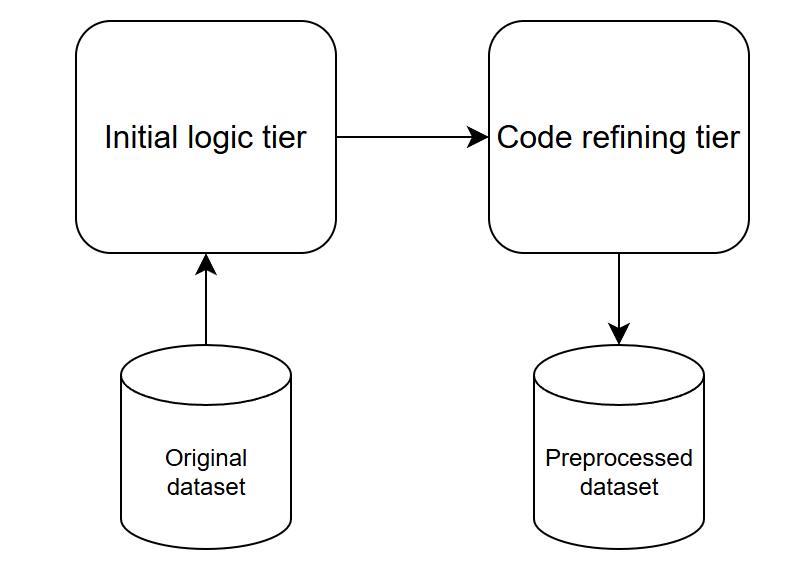
\includegraphics[width=0.5\textwidth]{media/image.png}
    \caption{Architecture of the Proposed Two-Tier Approach}\label{fig:architecture}
\end{figure}

By separating the preprocessing and code generation workflow into these two distinct phases, efficiency was maximized, potential error rates were reduced, and the output met the project's high standards of quality and functionality. This design provides a robust, scalable solution for automated data preparation, accommodating applications ranging from exploratory analyses to large-scale production environments where consistency and quality are essential.

\subsection{Evaluation Metrics}
To rigorously assess the effectiveness of the application, performance metrics focused on code accuracy, usability, and consistency were established. These include:
\begin{itemize}
    \item \textbf{Code Accuracy:} Measuring how accurately the generated code addresses the preprocessing requirements.
    \item \textbf{Usability:} Evaluating the code's readiness for direct use without extensive modifications.
    \item \textbf{Consistency:} Ensuring the application consistently produces reliable results across diverse datasets and preprocessing tasks.
\end{itemize}

\subsection{Testing and Validation}
To validate the application's functionality, tests were conducted using two representative datasets, covering a range of data types and preprocessing needs. These tests assessed the model's ability to generate correct and efficient code in line with the defined requirements, ensuring that the application met both performance and quality benchmarks. The testing phase verified that the application's output aligned with the quality objectives, confirming its readiness for deployment and real-world use.

\section{Mockup of the Application Interface}

\begin{figure}[H]
    \centering
    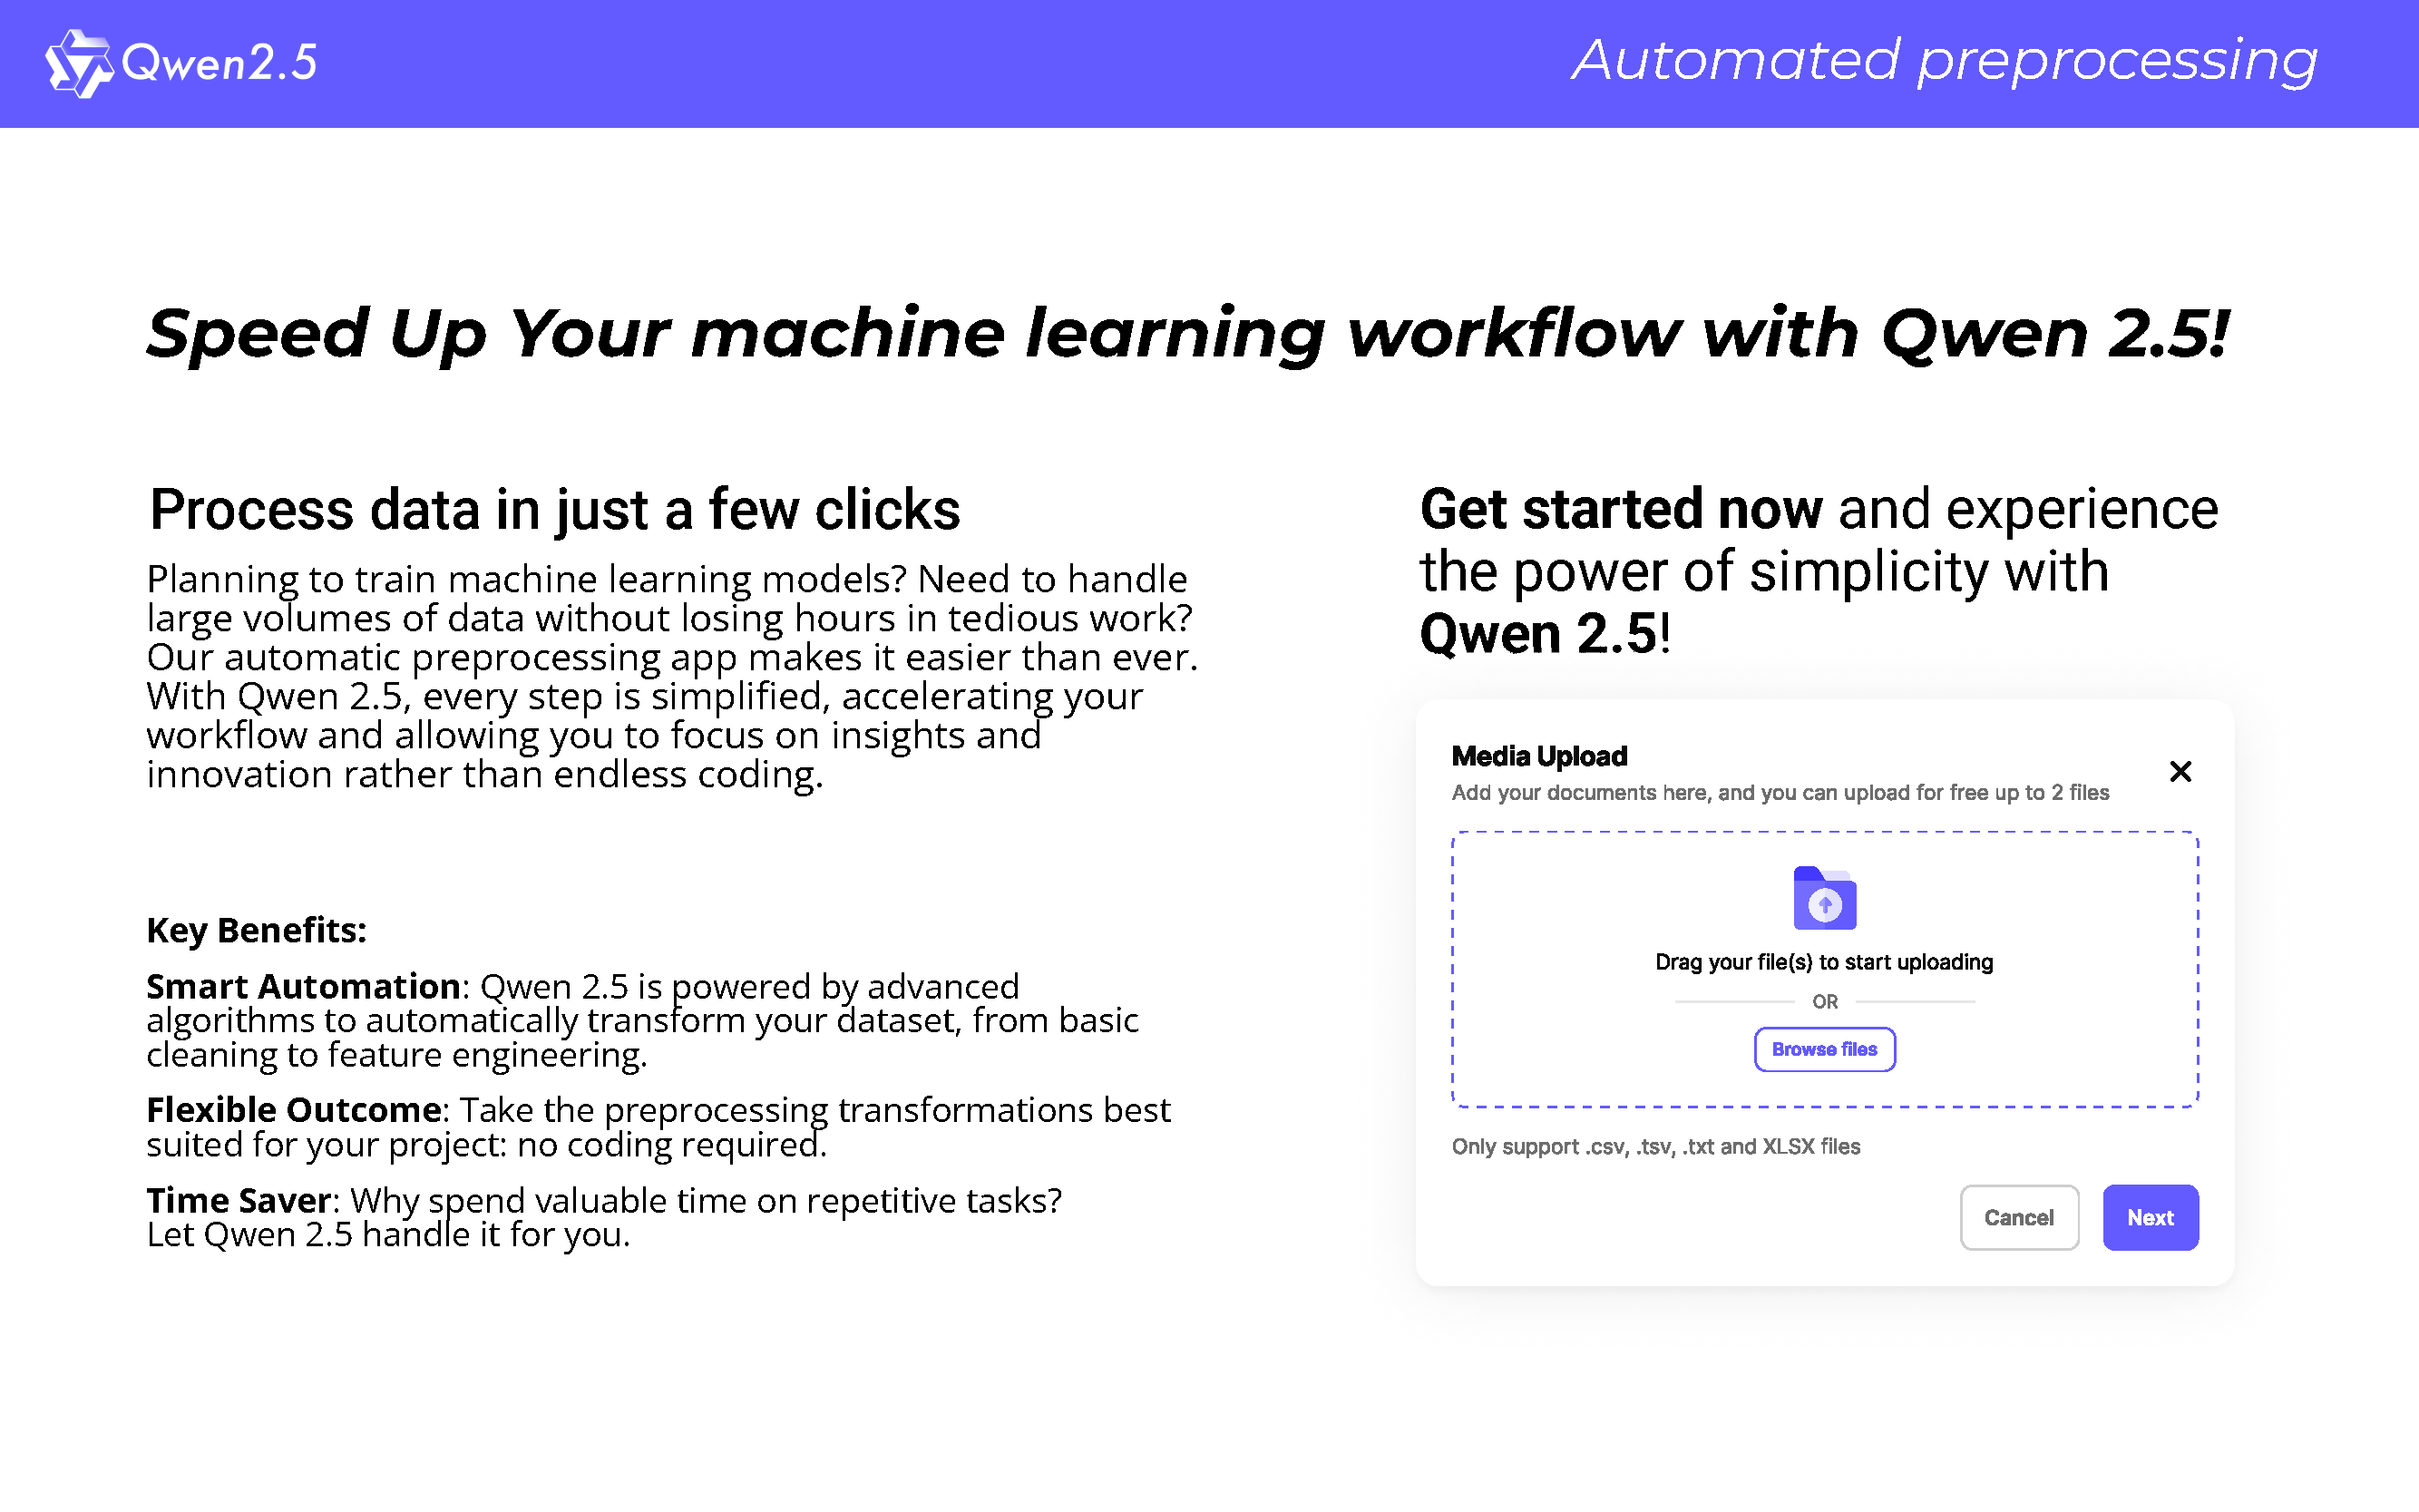
\includegraphics[width=1\textwidth]{media/App_prototipo_1.pdf}
    \caption{Main Page}\label{fig:app_mockup_1}
\end{figure}

\begin{figure}[H]
    \centering
    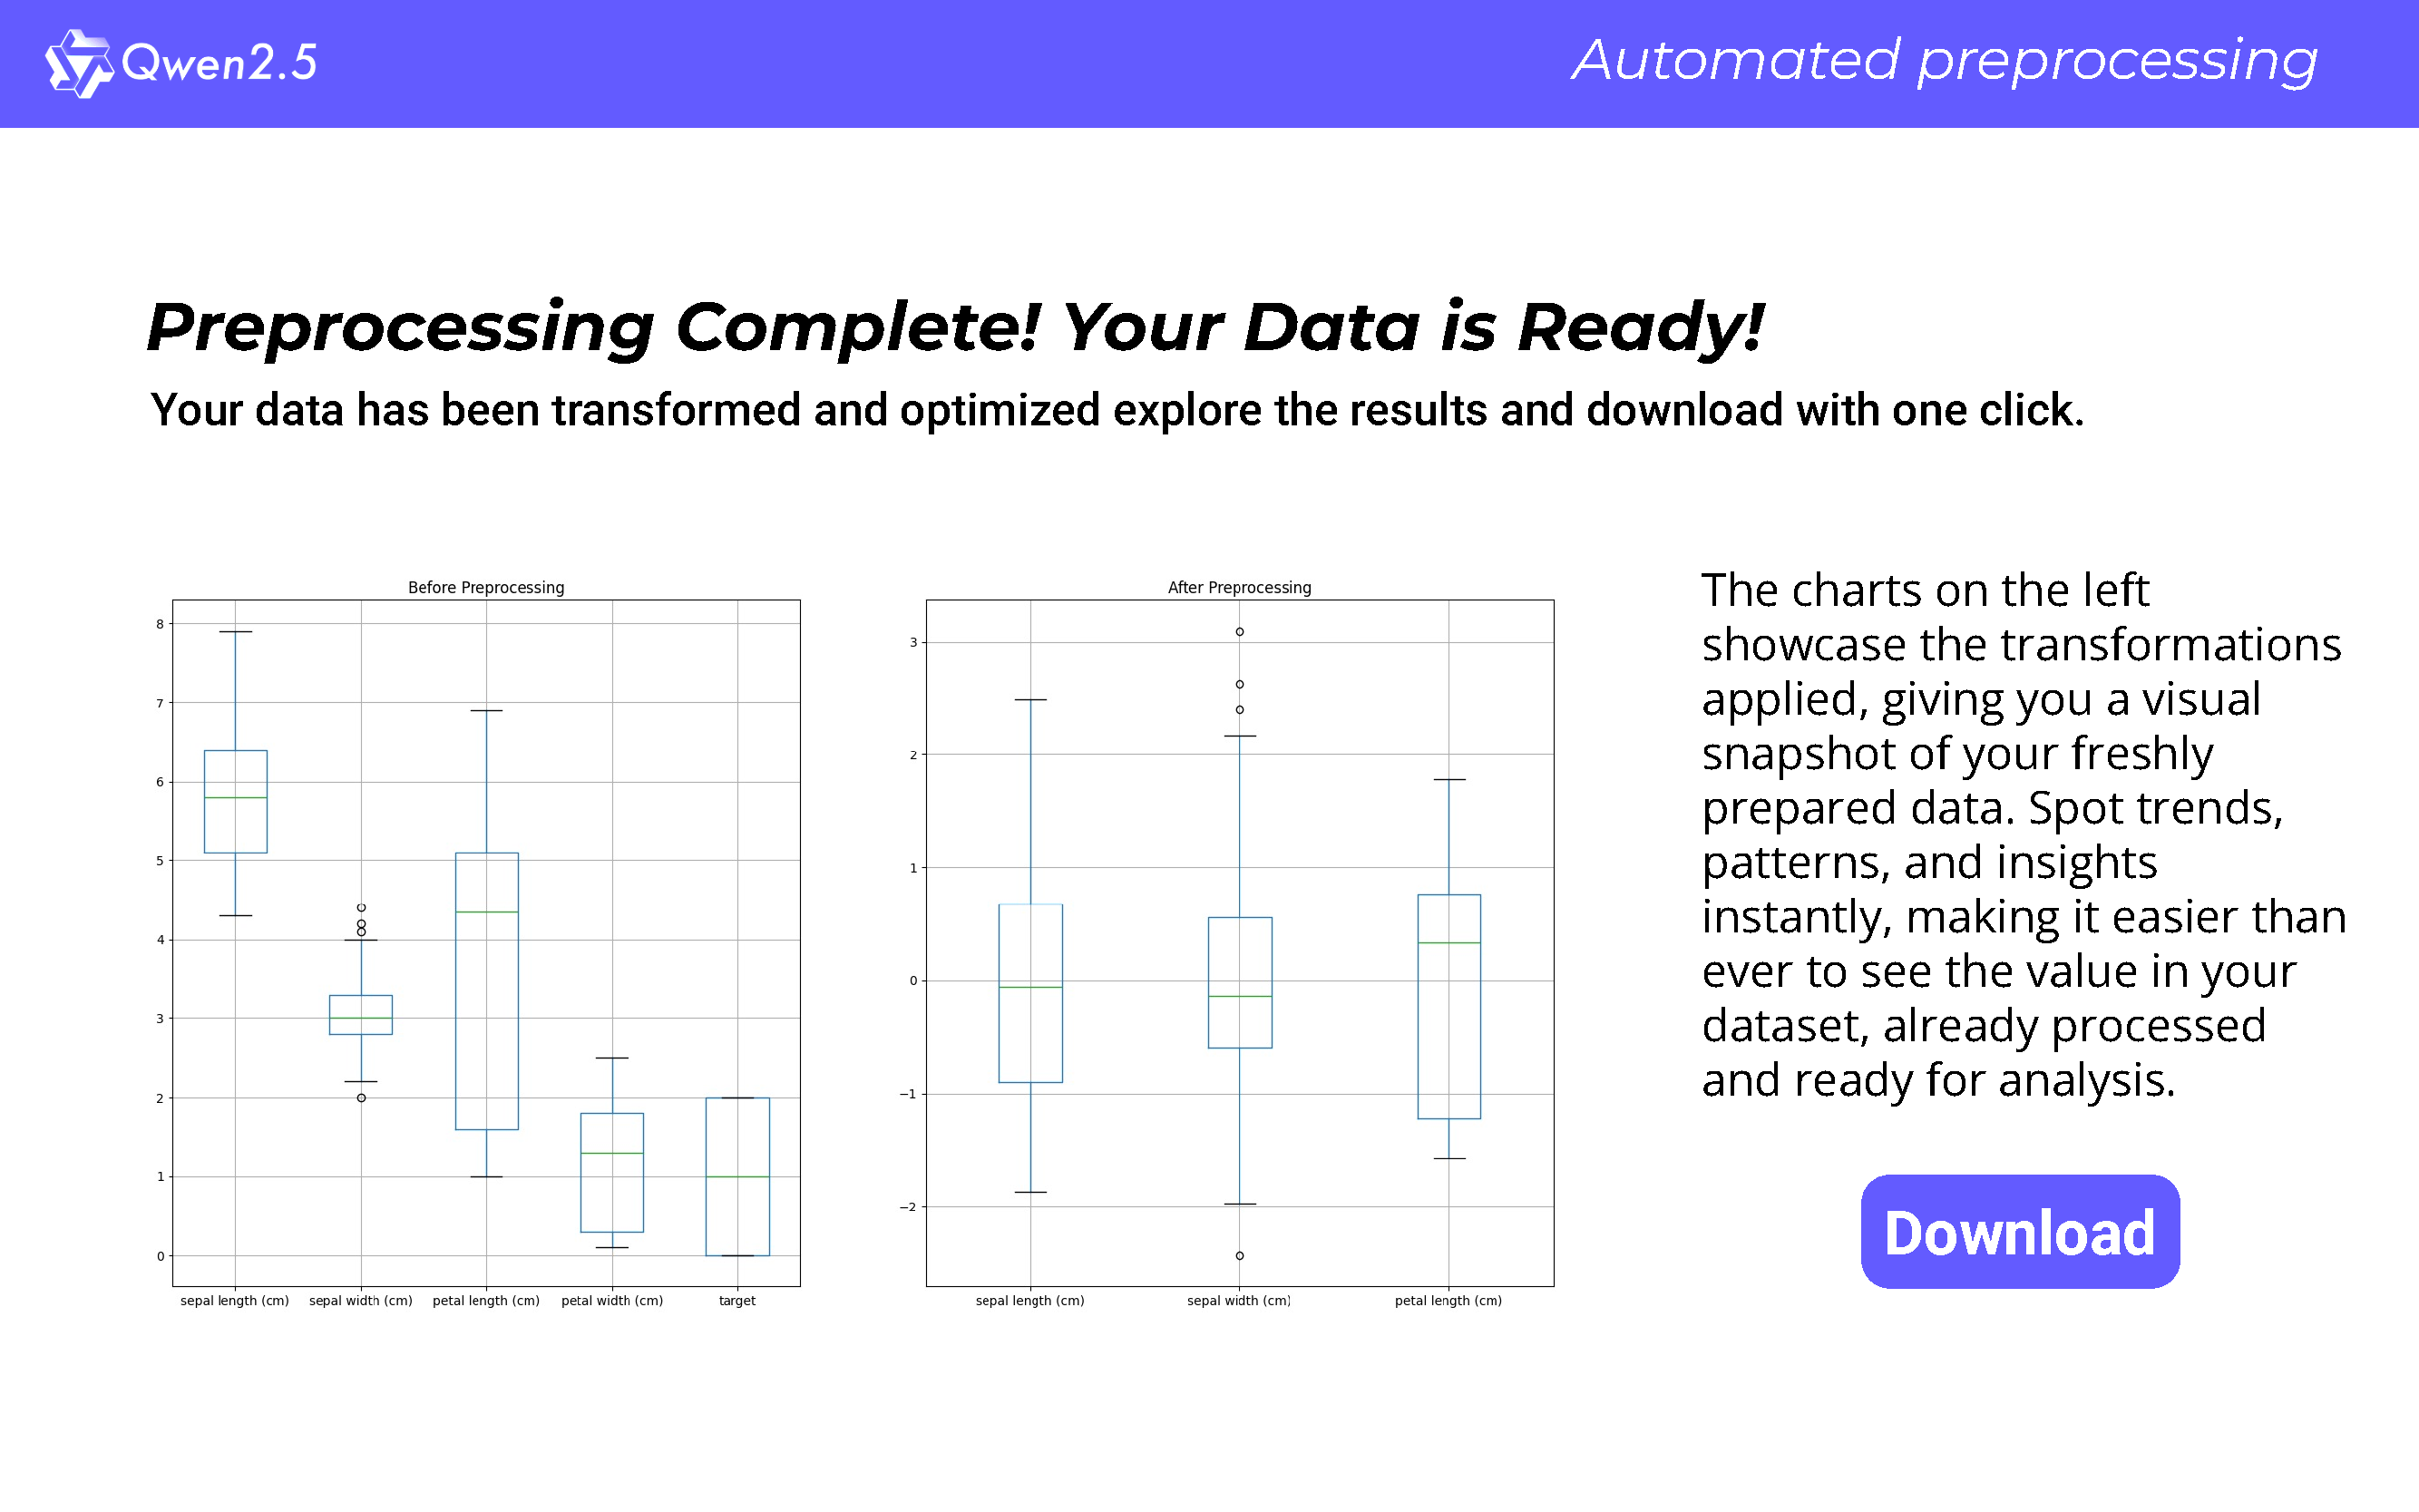
\includegraphics[width=1\textwidth]{media/App_prototipo_2.pdf}
    \caption{Results Page}\label{fig:app_mockup_2}
\end{figure}
\chapter{Results}
% \section{Preprocessing Comparisons}
% Several preprocessing methods were applied and compared across the two datasets used in this study. The \textit{House Prices} dataset, available from this \href{https://www.kaggle.com/competitions/house-prices-advanced-regression-techniques/data}{Kaggle link}, contains various features about houses and their prices, while the \textit{Iris} dataset provides measurements of iris flowers across different species.\\
% This study evaluated the preprocessing capabilities of the Qwen2.5 language model by applying it to two distinct datasets: the \textit{Iris} dataset, which contains exclusively numerical data, and the \textit{House Prices} dataset, which includes both numerical and categorical features. The primary objective was to identify the optimal preprocessing steps suggested by Qwen2.5 for each dataset.

\section{Preprocessing Comparisons}
This study compared several preprocessing methods across two datasets: the
\textit{House Prices} dataset from Kaggle, which includes various features
related to houses and their prices, and the \textit{Iris} dataset, which
contains measurements of iris flowers from different species. \\ The focus was
on evaluating the preprocessing capabilities of the Qwen2.5 language model. It
was applied to both datasets: \textit{Iris}, which is purely numerical, and
\href{https://www.kaggle.com/competitions/house-prices-advanced-regression-techniques/data}{\textit{House
        Prices}}, which features both numerical and categorical data. The goal was to
identify the most effective preprocessing steps for each dataset as suggested
by Qwen2.5.

After extensive testing, the best preprocessing outcomes generated by Qwen2.5
were selected. These results were then benchmarked against two established
preprocessing approaches:

\begin{enumerate}
    \item Preprocessing steps performed by our team and the Kaggle's users, specifically
          those rated as high-quality for each dataset.
    \item A parallel experiment using the LLaMA language model, in which identical
          preprocessing objectives and criteria were applied to ensure a fair comparison.
\end{enumerate}

The comparative analysis focused on multiple dimensions of preprocessing
performance, including the alignment of recommended steps with best practices,
the efficiency of data preparation, and the comprehensiveness in handling
missing values, scaling, encoding, and feature engineering. Additionally,
similarities and differences in the preprocessing pipelines across Qwen2.5,
Kaggle benchmarks, and the LLaMA model were examined to assess each model's
compatibility with established standards and adaptability to datasets with both
numerical and categorical features.

This section presents the findings from these comparisons, highlighting the
consistency, robustness, and adaptability of the preprocessing steps suggested
by Qwen2.5, relative to those obtained from experienced Kaggle practitioners
and the LLaMA model.

\subsection{House Prices Dataset}

\subsubsection{Comparison 1: Preprocessing by our Team}

The first step in preprocessing the \textit{House Prices} dataset involved
loading the dataset and examining its structure, which included analyzing the
features, data types, and missing values. This examination provided a clear
understanding of the data and informed the necessary steps for cleaning and
transformation.

The Id column was identified as irrelevant for the prediction model and was
removed from both the training and test datasets. The dataset was then split
into two parts: XX, representing the input features (excluding the target
variable, \textit{SalePrice}), and yy, the target variable \textit{SalePrice}.
Upon inspection, no duplicate rows were found, and therefore no action was
taken to remove any.

Outliers were identified through visual inspection by plotting
\textit{SalePrice} against \textit{GrLivArea}. Five extreme outliers were
detected and subsequently removed from the dataset to prevent distortion in the
model's performance.

Next, missing values in the numerical columns were addressed by imputing them
with the median value of the respective columns, ensuring no data were lost.
For some ordinal columns, where there were several unique values, similar
categories were grouped together to simplify the data and reduce complexity.

New columns were created by combining existing ones to reduce dimensionality
and potentially enhance the predictive power of the model. Only the most
relevant features, as determined by a correlation matrix, were retained for
further analysis.

Categorical columns were then encoded using One-Hot Encoding, ensuring they
were transformed into a numerical format suitable for machine learning
algorithms. Finally, numerical columns were scaled using the StandardScaler
method to standardize the features and ensure all variables were on the same
scale, facilitating better model convergence and performance.

\subsubsection{Comparison 2: Preprocessing by Alexandru Papiu}

Alexandru Papiu, a Kaggle user, applied preprocessing steps to the
\textit{House Prices} dataset. The notebook can be found in this
\href{https://www.kaggle.com/code/apapiu/regularized-linear-models}{Kaggle
    link}.

In order to make the distribution of skewed features more "normal" (selecting
those with skew > 0.75) the target variable (SalePrice) is transformed to
reduce skewness and make it more normally distributed using a log
transformation.

Then, dummy variables are created for categorical features using to transforms
categorical data into a format suitable for machine learning algorithms, where
each unique category becomes a separate binary feature.

After this, numeric features with missing values (NaN) are replaced with the
mean of their respective columns. This step ensures that no data points are
missing and that all columns have valid values for subsequent modeling.

Before and after transformations, histograms are plotted to visualize the
effect of the log transformation on SalePrice. This step helps demonstrate how
the transformation makes the distribution more normal.

The combined dataset is split back into training and testing feature sets. The
target variable (y) is extracted as the transformed SalePrice. This step
prepares the data for input into a machine learning model.

\subsubsection{Comparison 3: Preprocessing by Erik Bruin}

Another Kaggle user, Erik Bruin, has done preprocessing on the \textit{House
    Prices Dataset} at the following
\href{https://www.kaggle.com/code/erikbruin/house-prices-lasso-xgboost-and-a-detailed-eda}{kaggle
    link}.

The code first identifies columns with missing values (NA) and counts the
number of NAs for each column. This step allows a clear understanding of where
data is missing and how extensive the issue is.

The code works through the 34 predictors with missing values, starting from the
ones with the most NAs and addressing each systematically. Related variables
(e.g., Pool, Garage, Basement) are handled together when they form logical
groups.

Remaining character variables (non-numeric) are identified and processed. If
there is a clear order or hierarchy (ordinal data), they are encoded as ordinal
integers.

Where appropriate, variables are label-encoded or converted into one-hot
encoded features to prepare them for machine learning models.

Ordinal values are encoded using an ordinal scale for consistent ordering.

All NA values are filled or handled, ensuring complete data. Character and
numeric variables are converted into appropriate formats (factors, label
encoding, etc.) for further analysis.

Categorical variables are properly encoded for machine learning algorithms.

\subsubsection{Comparison 4: Automation of Data Preprocessing with LLaMA}

In this test, the LLaMA (version 3.2-Vision:11b) model was used to automate the
data preprocessing workflow. The task involved providing an unprocessed input
dataset and instructing LLaMA to generate a Python script that would perform
basic preprocessing tasks such as data cleaning, normalization, and encoding of
categorical variables.

Two specific prompts were used to guide LLaMA's output. The first (Level 1)
instructed LLaMA to analyze the dataset descriptor and identify necessary
preprocessing steps. The second (Level 2) asked LLaMA to generate Python code
to perform these preprocessing operations directly on the dataset.

Although LLaMA generated Python code based on these prompts, the resulting
script contained several errors and required human intervention to correct.
Some preprocessing steps also needed refinement for optimal performance.
Despite these challenges, the test demonstrated LLaMA's potential in automating
certain preprocessing tasks, though human oversight remained essential to
ensure the final script met the required standards.

\begin{figure}[H] 
    \centering 
    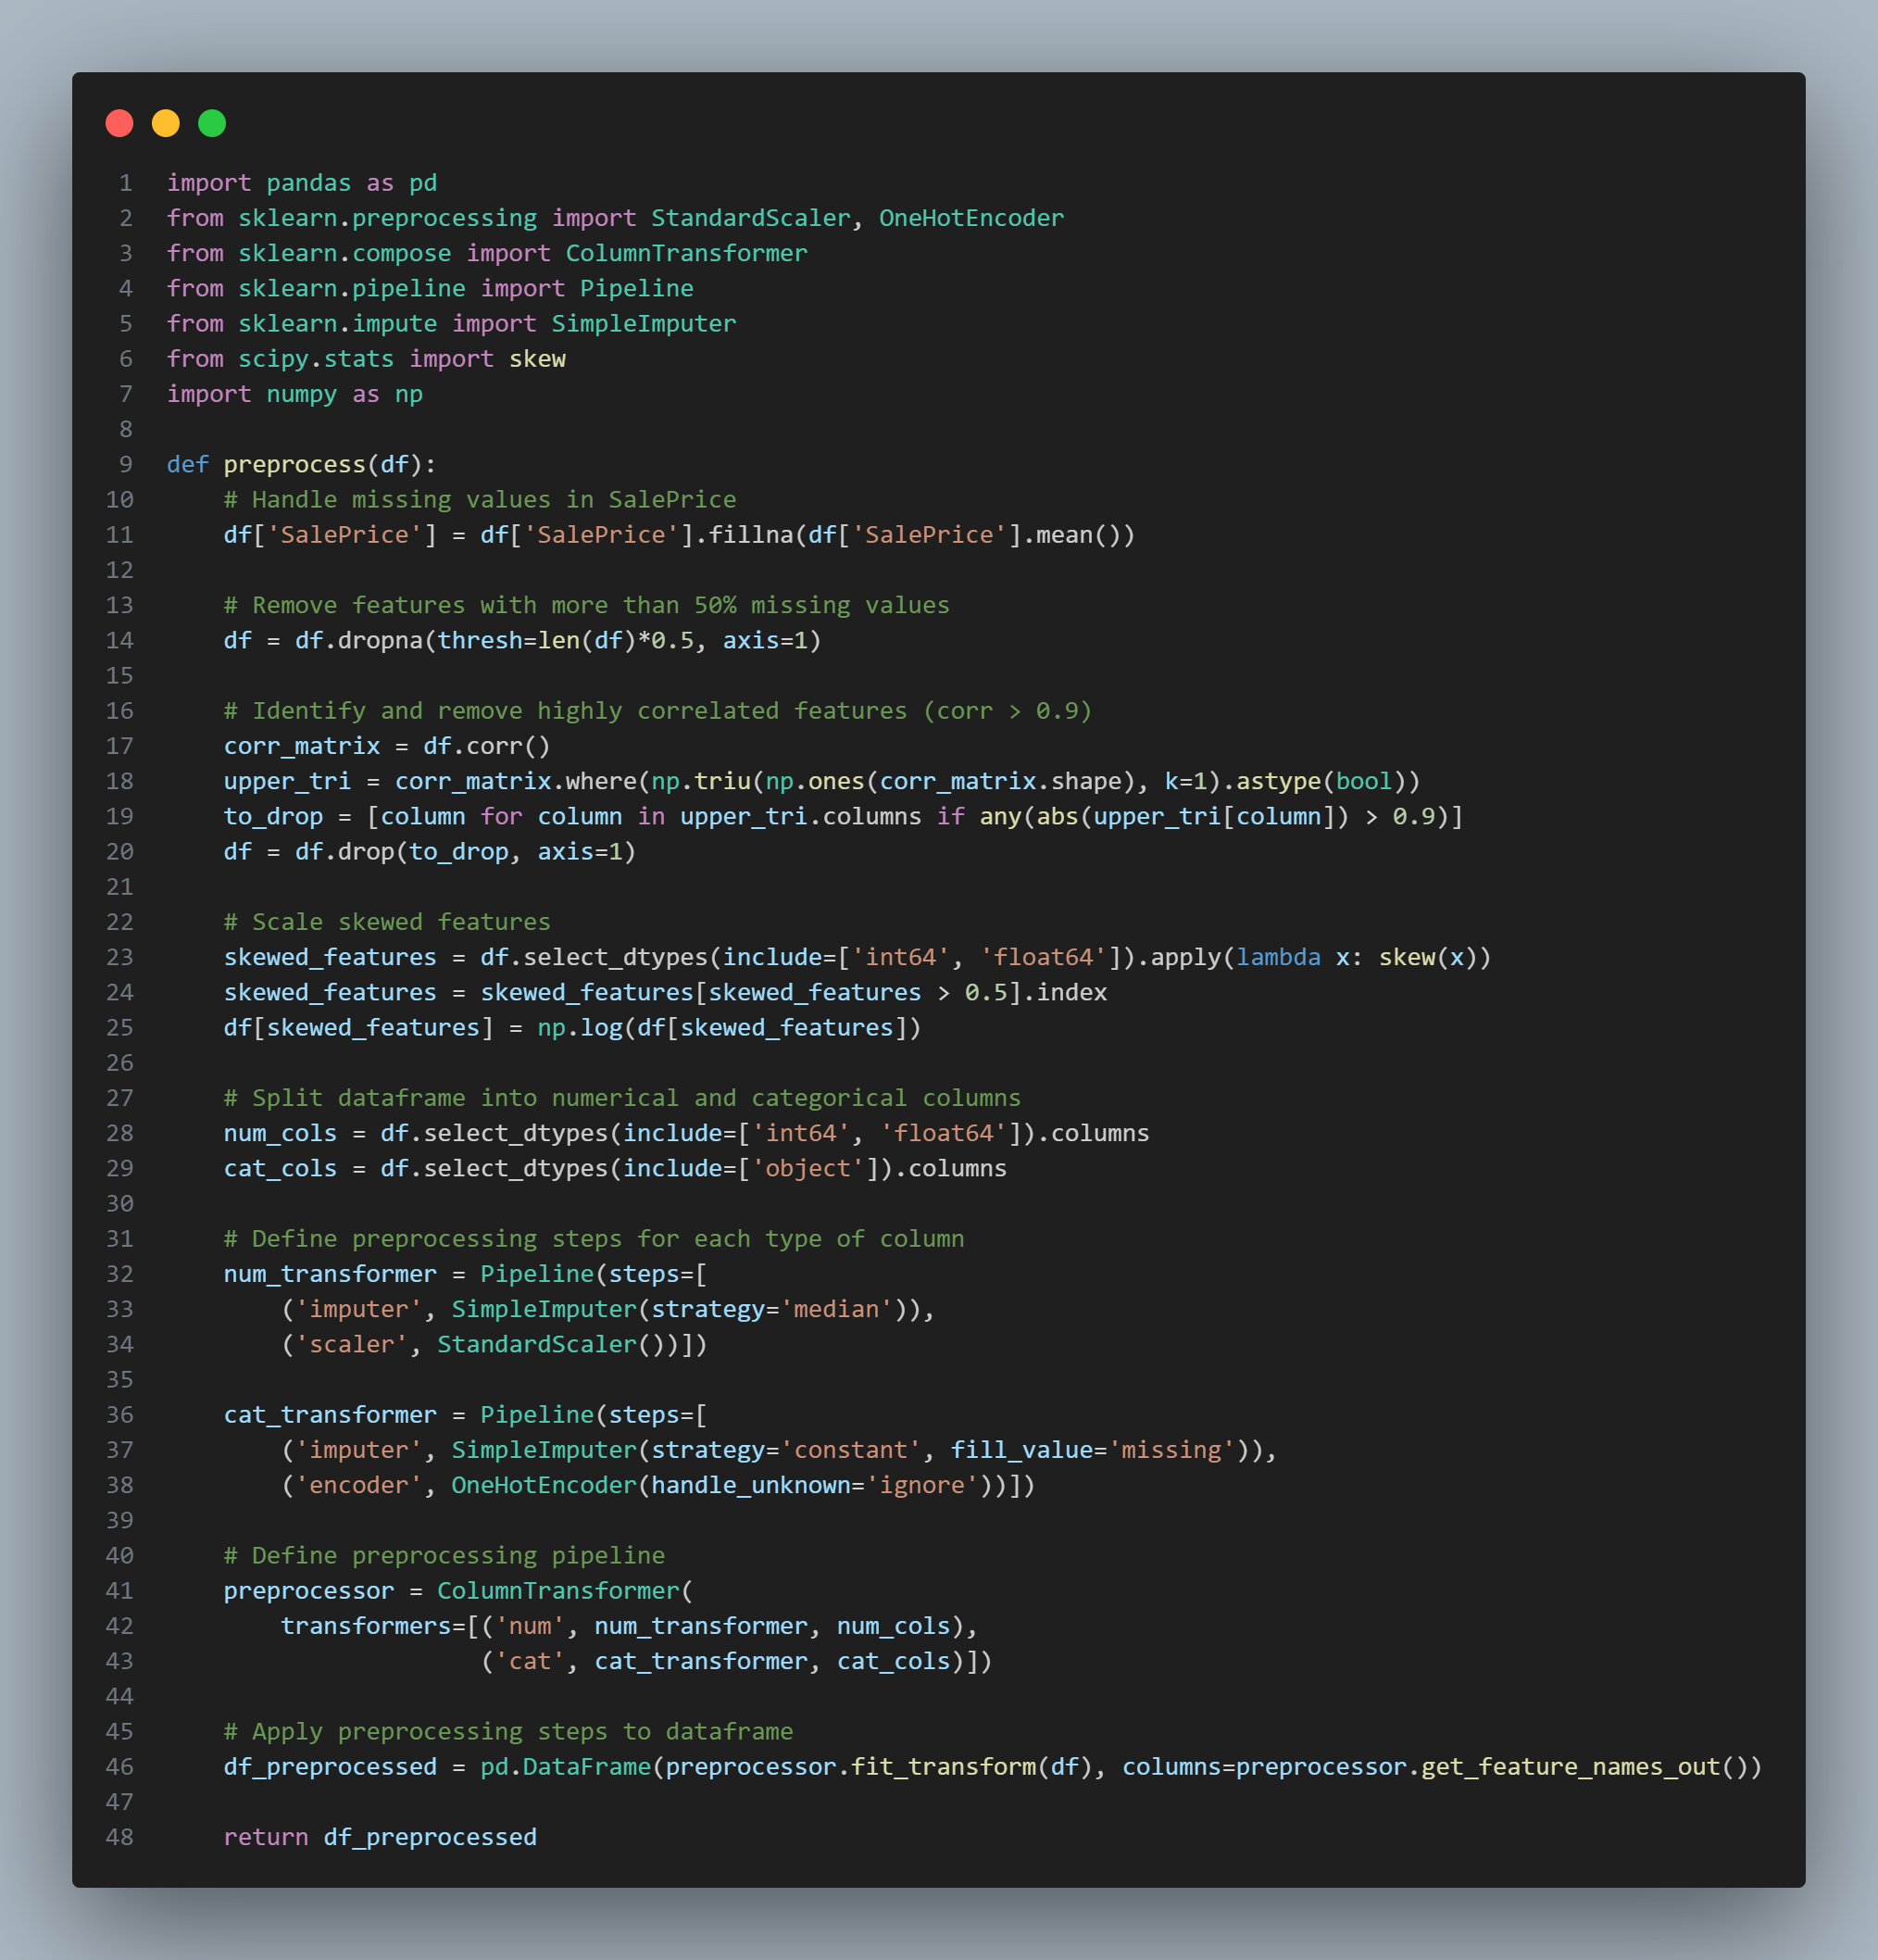
\includegraphics[width=0.7\textwidth]{media/LlamaCode.png} 
    \caption{Example of preprocessing script generated by LLaMA} 
\end{figure}

The use of \textit{role prompting} or \textit{persona prompting} in the
prompts, such as \textit{"You are a data engineer skilled in artificial
    intelligence..."} was particularly effective. This approach guides the LLM to
assume a professional role, focusing on the relevant aspects of the task and
tailoring responses to suit the context. This method helped in generating more
focused, accurate responses, minimizing ambiguity, and optimizing the overall
efficiency of the generated code.

\subsubsection{Our Approach: Application-Driven Preprocessing by Qwen2.5}

Multiple trials were run with varying prompts to assess the model's
effectiveness under different conditions. While the results showed promise,
they were slightly behind those achieved through other technologies or manual
methods, requiring several attempts to get acceptable performance.

Although still in development and dependent on current computational resources,
the application demonstrated clear potential for future improvement. While the
results were not perfect, they were encouraging, indicating that with
advancements in computational power and algorithm optimization, performance and
efficiency could be significantly enhanced.

\begin{figure}[H]
    \centering
    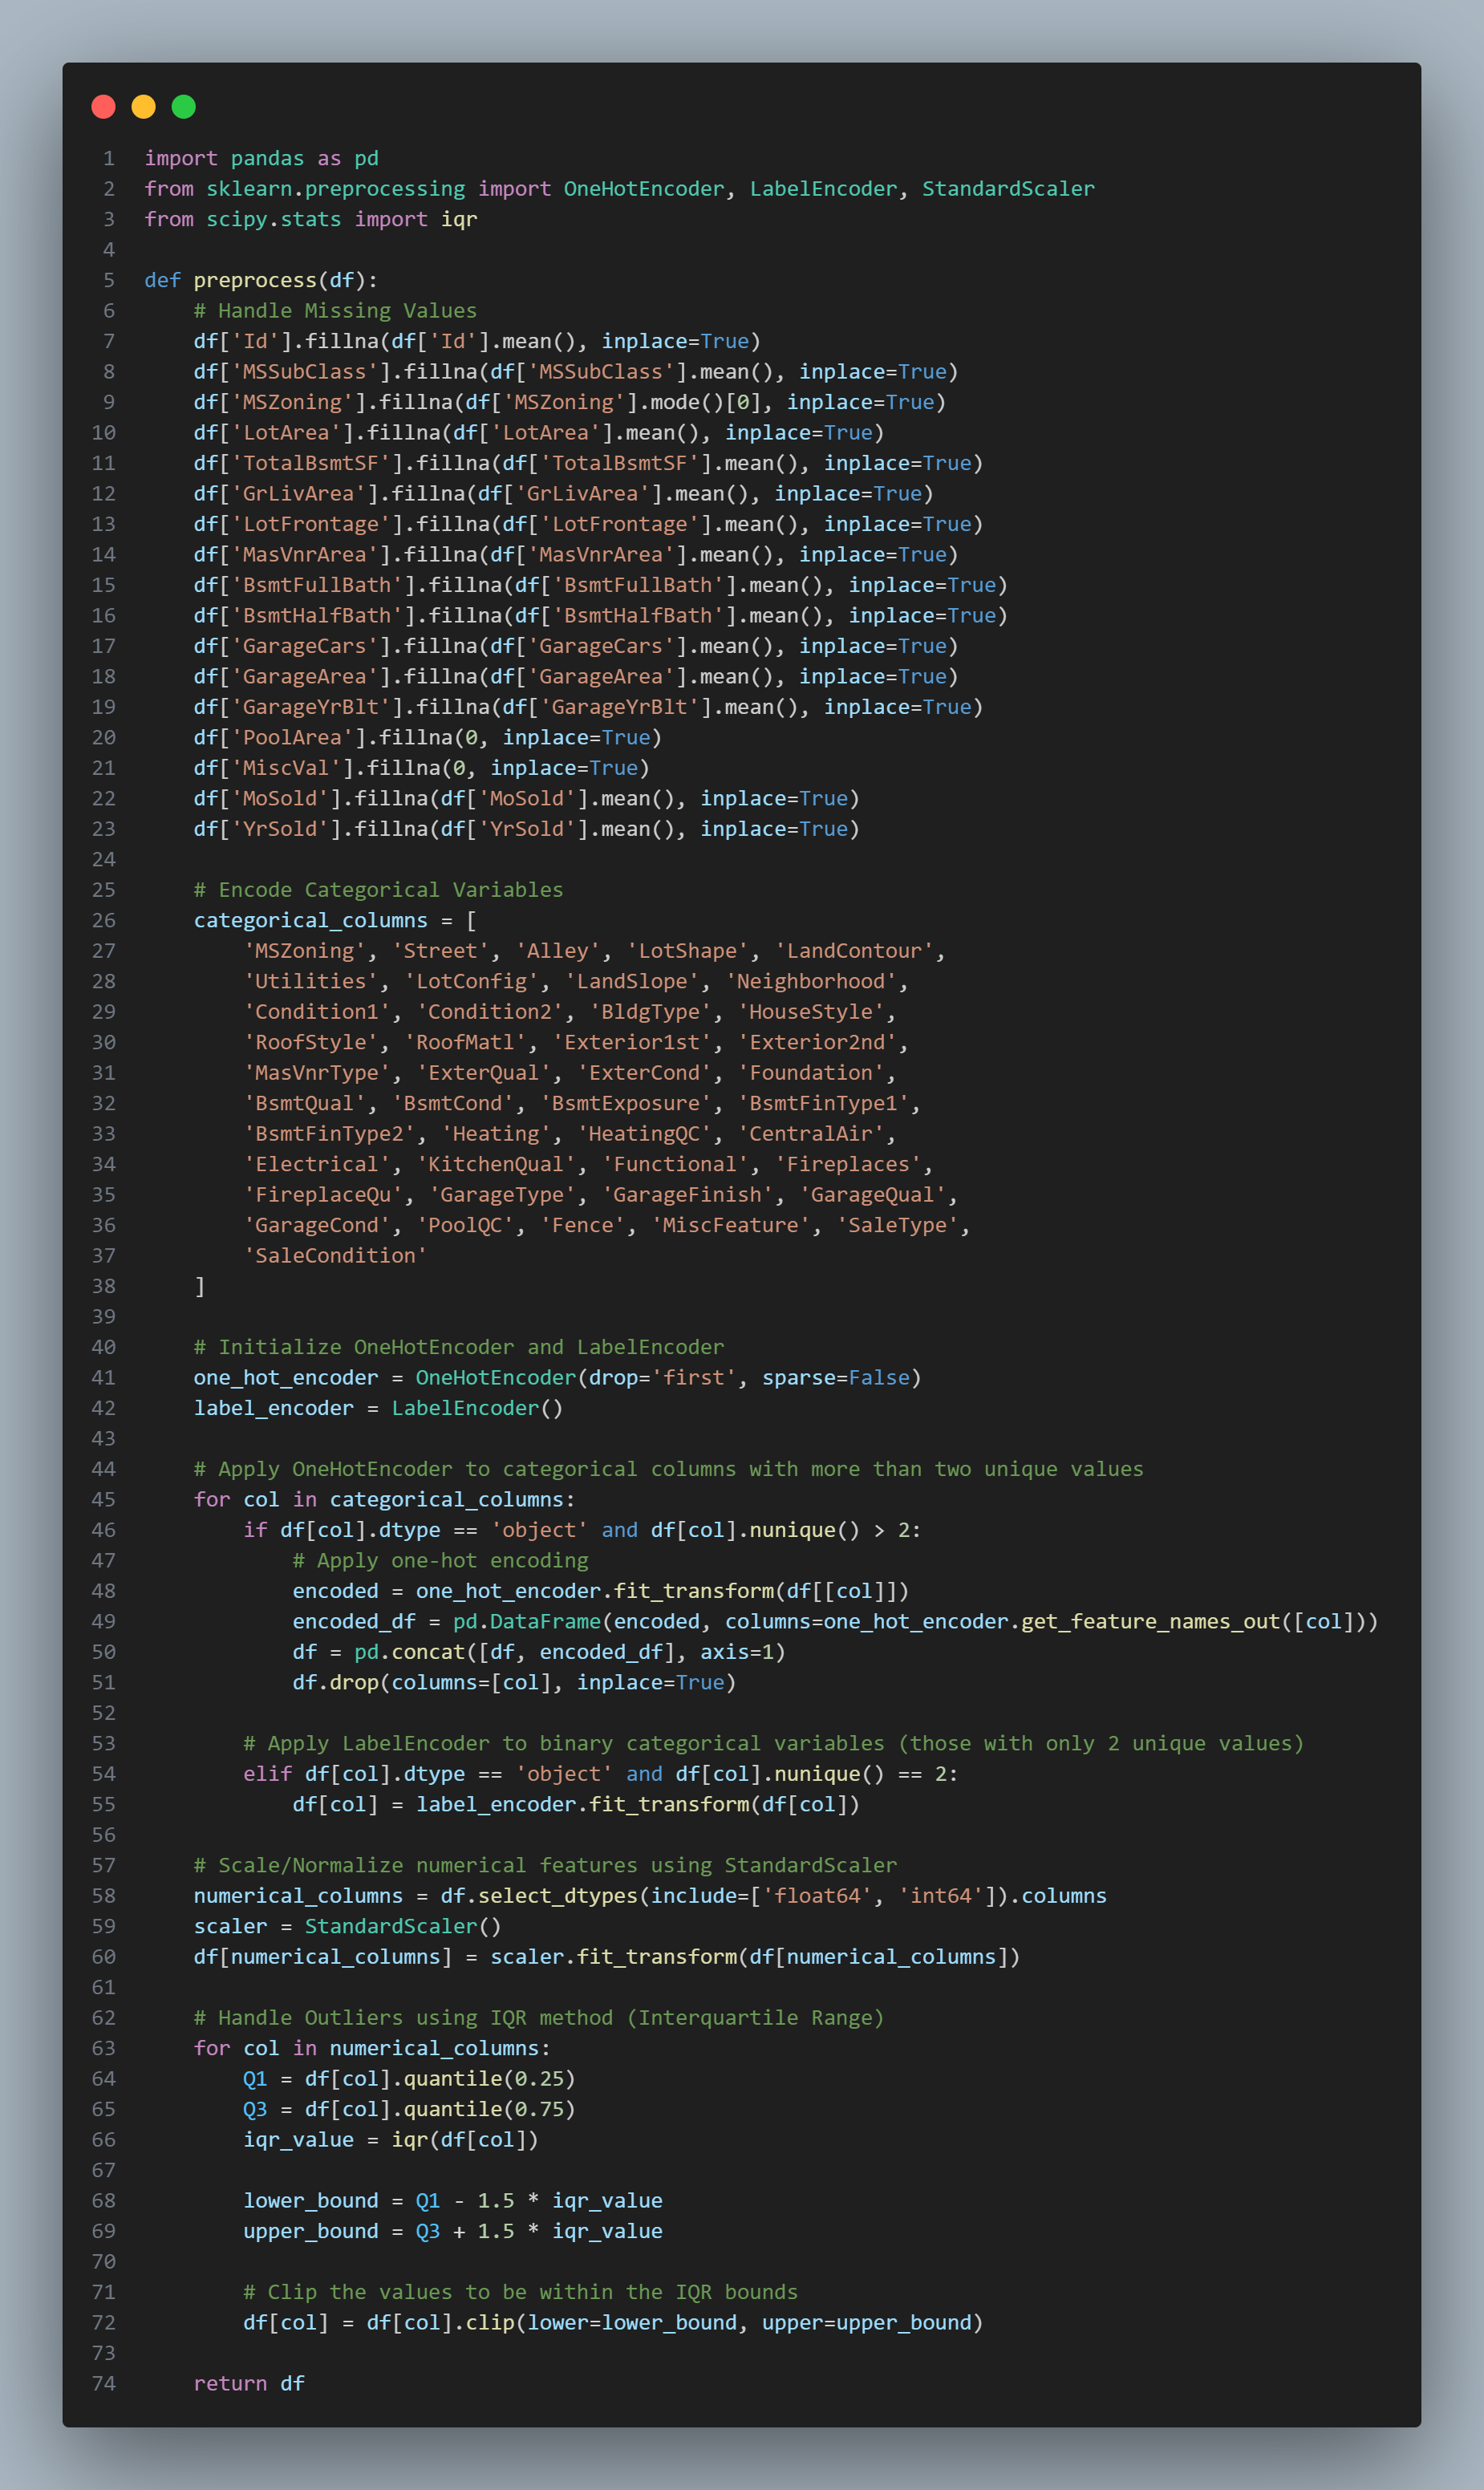
\includegraphics[width=0.9\textwidth]{media/Qwen2.5code.png}
    \caption{Example of preprocessing script generated by Qwen2.5}
    \label{fig:application-driven-preprocessing}
\end{figure}

\newpage
\subsection{Iris Dataset}

\subsubsection{Comparison 1: Preprocessing by Shoukat Khan}
This example is given by user Shoukat Khan in the following
\href{https://www.kaggle.com/code/drisrarahmad/iris-flower-dataset}{Kaggle
    link}. First thing the user did was to visualize the dataset information. After
this, the `Id' column was dropped, as it was considered unnecessary for the
future analysis of the dataset. Then some exploratory analysis was done to show
the relationships between the different features of the dataset and how they're
distributed. Then he checked the presence of null values in the dataset, but
none were found. The numerical features were then scaled using the
StandardScaler method. Finally, the dataset was split into training and testing
sets for further analysis.

\subsubsection{Comparison 2: Preprocessing by Our Team}
The Iris dataset was preprocessed by our team using a structured approach. The
dataset was loaded and examined to understand its structure and features. The
`Id' column was identified as irrelevant and removed from the dataset. The
dataset was then split into input features (X) and target variable (y). No
duplicate rows were found, so no action was taken to remove any. Missing values
were checked, but none were present in the dataset. The numerical features were
scaled using the StandardScaler method to standardize the data.

\subsubsection{Comparison 3: Preprocessing the Iris Dataset with Llama}

The Iris dataset was also preprocessed using Llama (version 3.2-Vision:11b). As
with the House Prices dataset, we provided Llama with structured prompts to
guide the preprocessing steps. However, given the relative simplicity of the
Iris dataset (with fewer features and minimal missing data) preprocessing was
more straightforward, enabling Llama to generate more accurate and usable
Python code.

For this dataset, we observed that Llama required fewer corrections compared to
the more complex House Prices dataset. The generated code effectively addressed
essential preprocessing tasks, including handling categorical data, normalizing
numerical features, and managing any missing values, though such issues were
limited in the Iris dataset.

\begin{figure}[H]
    \centering
    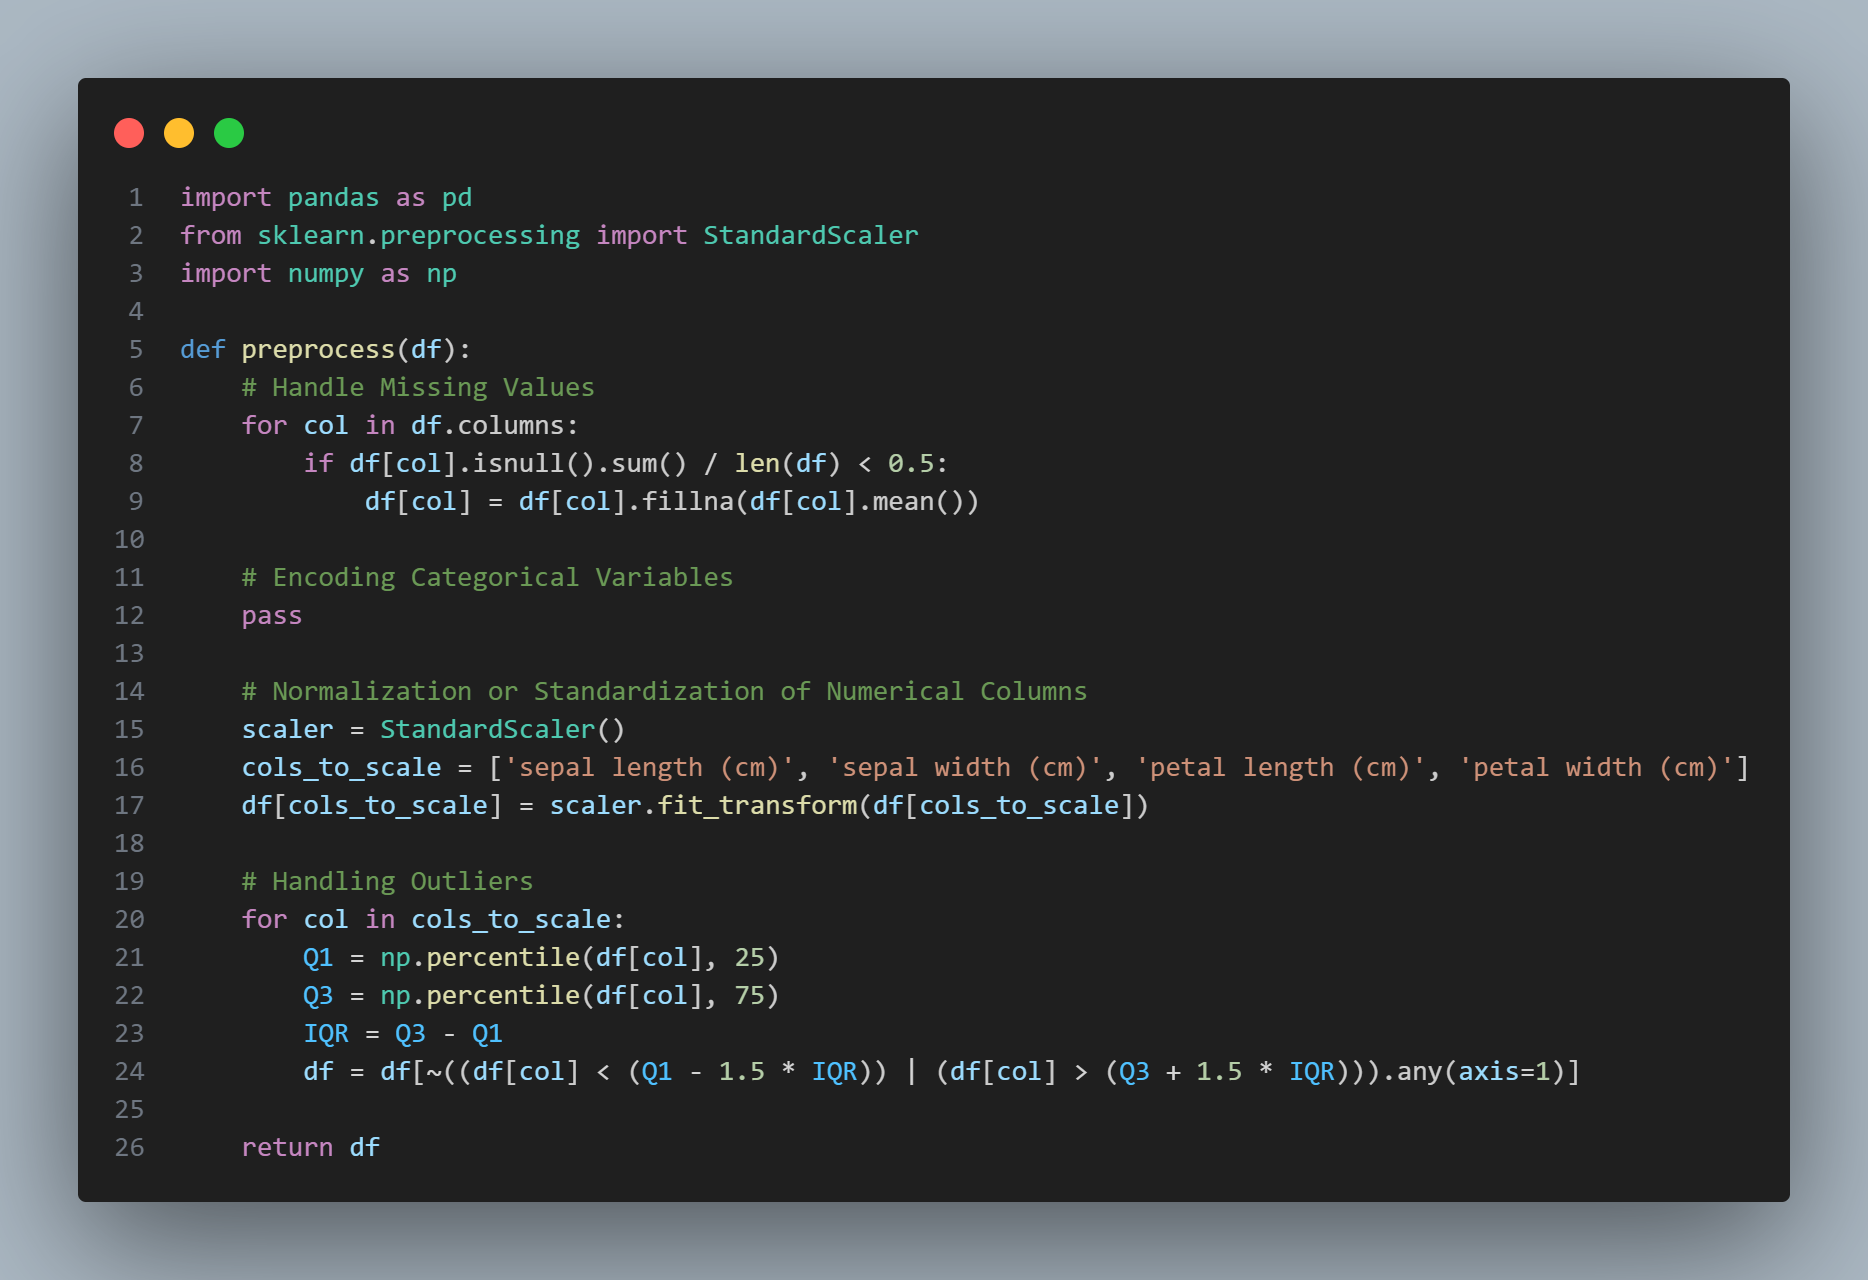
\includegraphics[width=0.7\textwidth]{media/IrisCode.png}
    \caption{Example of preprocessing script generated by LLaMA for the Iris dataset}
    \label{fig:llama-code-iris}
\end{figure}

\subsubsection{Our approach: Application-Driven Preprocessing by Qwen2.5}

Our application was also used to preprocess the Iris Dataset. Performance on
this dataset exceeded that of the House Prices dataset, which is significantly
more complex. This suggests that our application is particularly effective for
simpler datasets like Iris, while it becomes more challenging to implement on
larger and more diverse datasets.

The primary limitation lies in the model's inability to perform independent
training. Without the capability to learn autonomously, the model relies on
predictions based solely on previously observed data. Consequently, it performs
better with simpler datasets, where fewer details must be processed, allowing
for more accurate predictions. These findings indicate that the model has
considerable potential and could yield more accurate results and achieve
complete automation of data preprocessing with increased data and computational
power.

\begin{figure}[H]
    \centering
    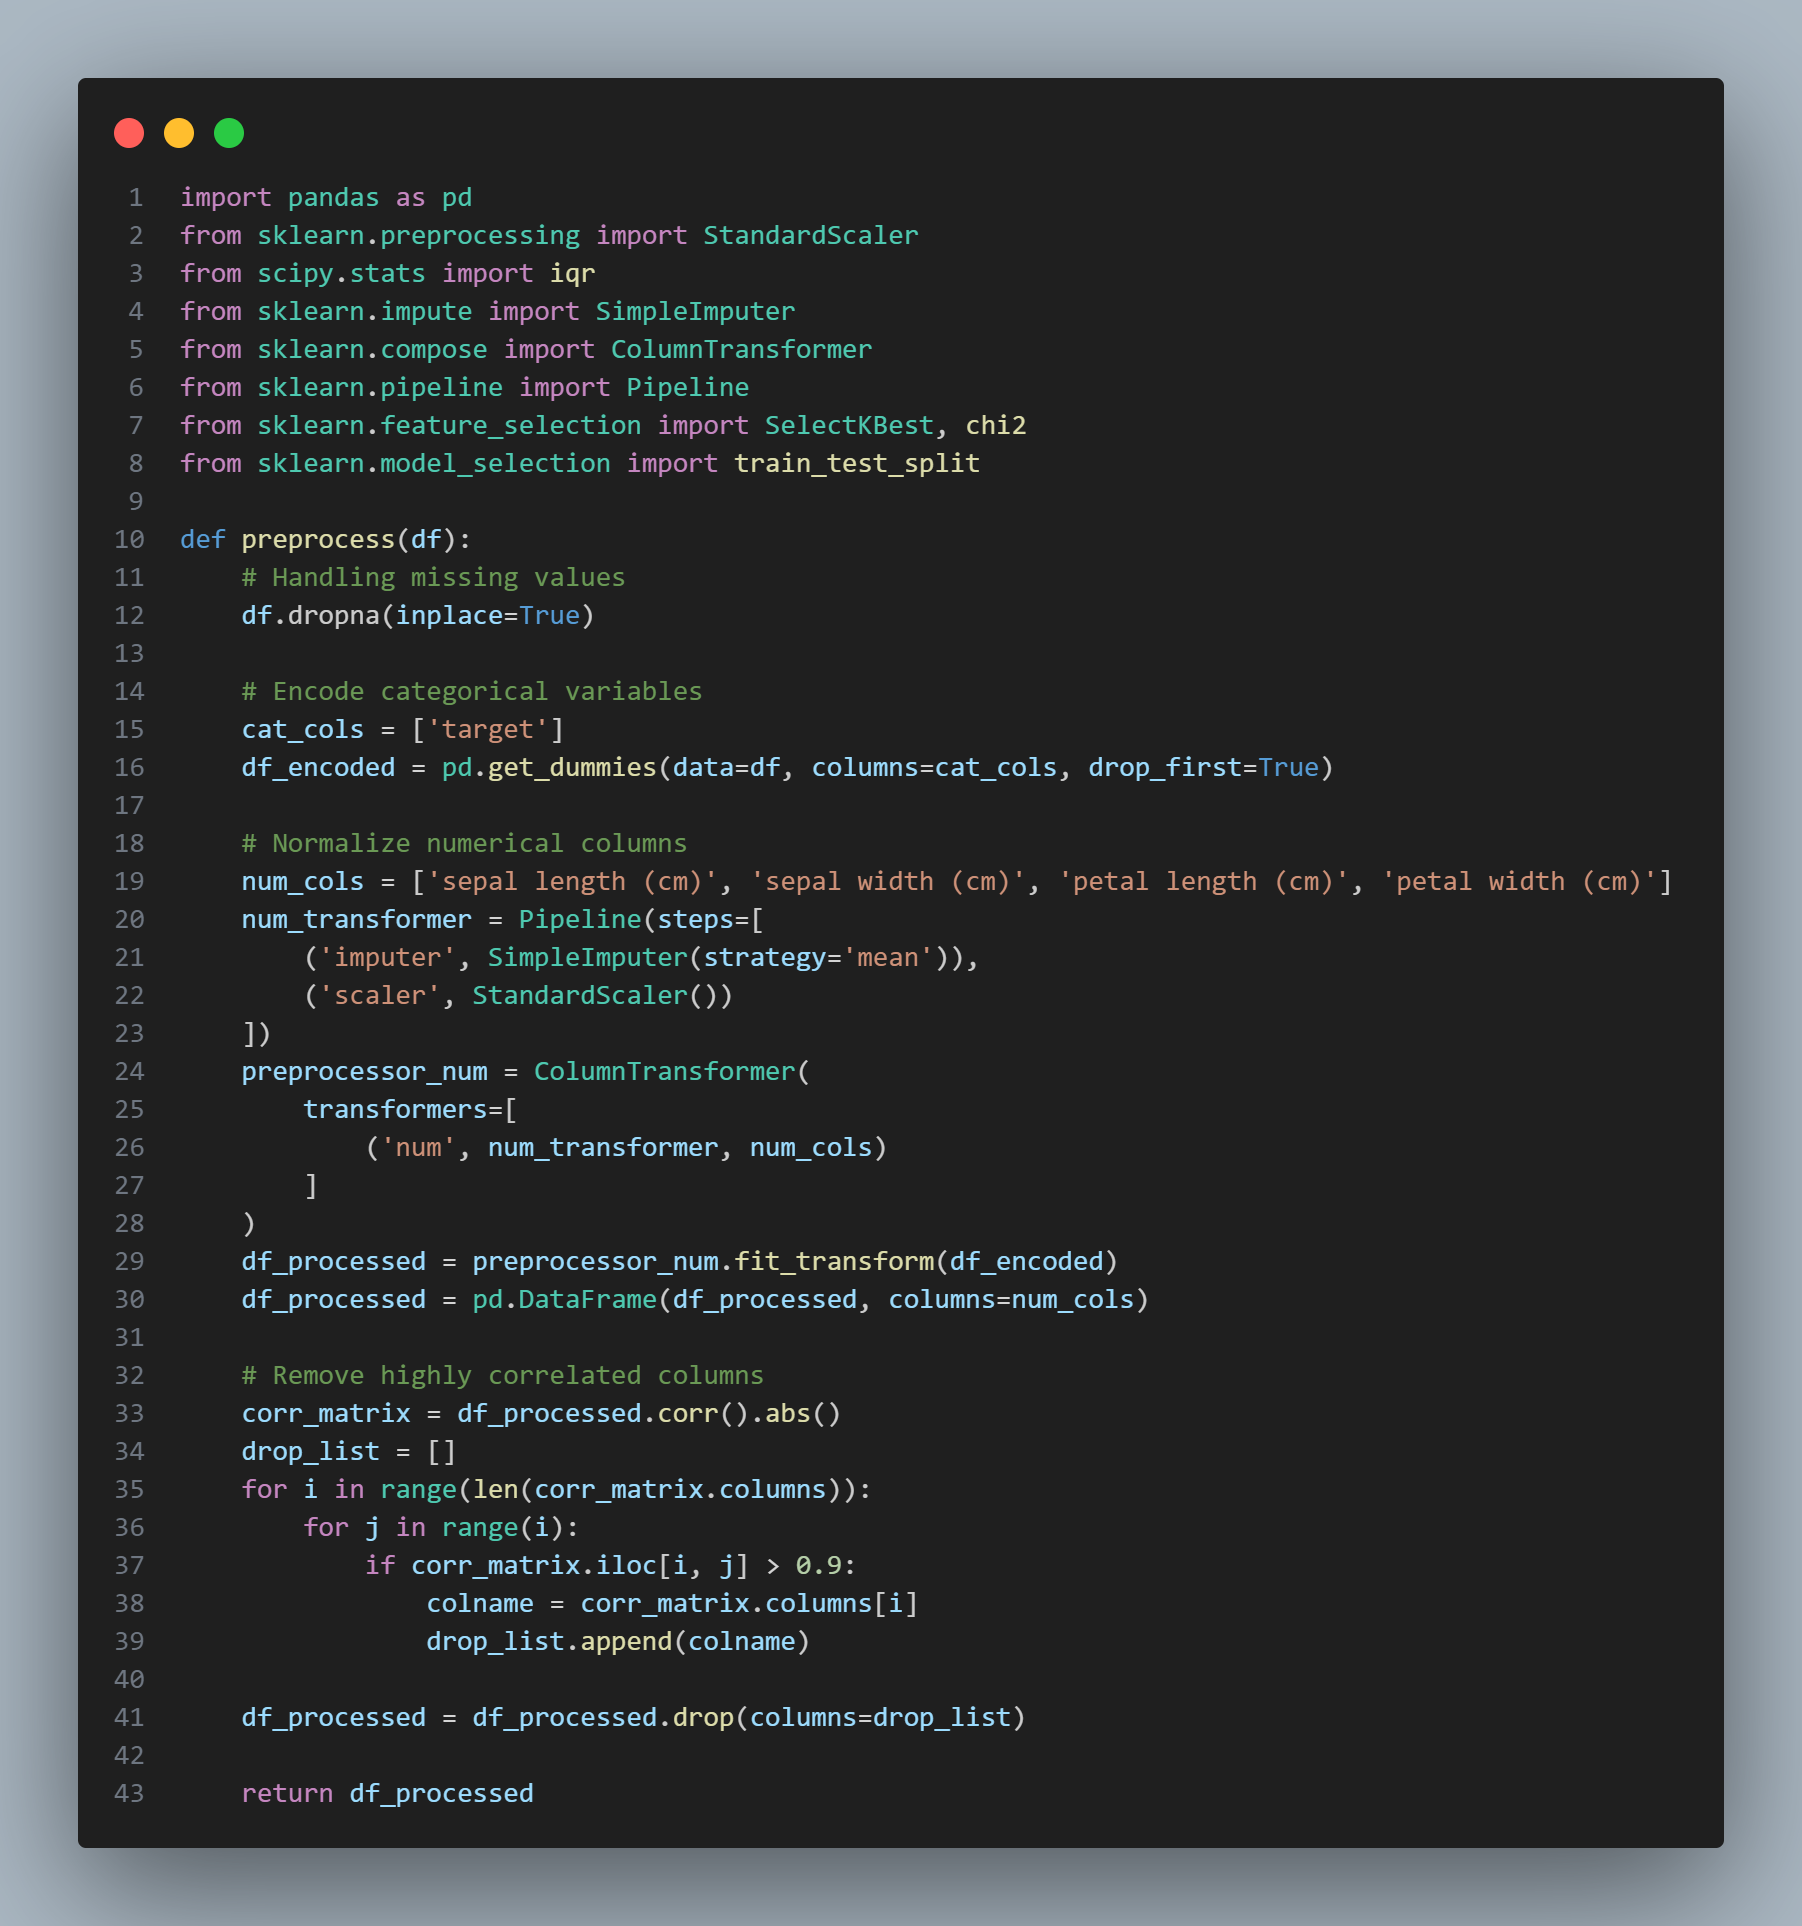
\includegraphics[width=0.7\textwidth]{media/Qwen2.5codeIRIS.png}
    \caption{Example of preprocessing script generated by Qwen2.5 for the Iris dataset}
    \label{fig:application-driven-preprocessing-iris}
\end{figure}

\subsection{Performance comparison}

% \subsubsection{House Prices Dataset}

% All the \textbf{manual approaches} carefully identify and impute missing data,
% ensuring no data loss while maintaining data integrity. Different imputation
% strategies are used based on context, with median or mean imputation for
% numerical features and domain-driven values for categorical features. They all
% transform categorical variables into numerical formats through one-hot
% encoding, label encoding, or factorization. This ensures that the data is in a
% form suitable for machine learning models. Alexandru Papiu and Erik Bruin
% emphasize encoding of ordinal features using ordinal integers when applicable,
% demonstrating consistency in preprocessing steps for such data types. Outliers
% are identified and removed, and distributions of target and input features are
% analyzed (e.g., via visual inspection). Both our team and Erik Bruin utilize
% exploratory analysis, such as plotting distributions, to better understand data
% trends and relationships between features.

% Alexandru Papiu applies a log transformation to the target variable (SalePrice)
% to reduce skewness, aligning it more closely with a normal distribution. The
% Team's approach involves standardizing numerical features using StandardScaler,
% a common practice to improve model convergence. This step was not mentioned in
% the summaries of the other manual approaches but remains a potential
% consideration for enhancing the comparability of numeric inputs.\\

% Both \textbf{AI-driven approaches} involve automated code generation based on
% input prompts, leveraging the capabilities of large language models (LLMs) to
% understand and perform preprocessing tasks. The use of role prompting in LLaMA
% guides it to generate tailored responses, demonstrating the value of carefully
% constructed prompts in directing AI behavior.

% The AI approaches automate typical preprocessing tasks such as imputation,
% normalization, and encoding of categorical variables. The focus on basic data
% cleaning, normalization, and transforming features for compatibility with
% machine learning models shows their potential to streamline preprocessing
% tasks.\\

% Manual approaches demonstrate a nuanced understanding of data context. For
% example, Erik Bruin groups related features for handling (e.g., Pool, Garage,
% and Basement), applies specific imputation strategies based on domain
% knowledge, and tailors transformations according to feature distributions.
% AI-driven methods tend to follow generalized rules or learned heuristics, which
% may not account for specific domain considerations without further tuning and
% guidance.

% Manual methods allow for fine-tuning based on data insights gained from
% exploration, such as identifying and removing outliers, specific imputation
% strategies, and encoding schemes tailored to data distributions. AI-driven
% methods like LLaMA often require human intervention to refine the generated
% code, demonstrating limitations in achieving optimal solutions without manual
% oversight.

% AI approaches offer a faster, automated process for generating initial
% preprocessing scripts, reducing the amount of repetitive work required by data
% scientists. This can be highly beneficial for rapid prototyping. Manual
% approaches are more time-consuming but can be more precise due to direct human
% involvement and domain knowledge.

% Manual methods generally exhibit fewer errors because they leverage human expertise to identify and address issues during each preprocessing step. In contrast, AI-driven preprocessing, such as that performed by Qwen2.5, often produces code that can be suboptimal or contain errors without substantial human refinement. In our experiment, the LLM's output was often insufficiently accurate, remaining overly generic and requiring numerous iterations to yield a functional solution. Even then, the results fell short of the quality expected for reliable preprocessing. This highlighted a significant gap in the model's ability to autonomously make effective decisions, underscoring the need for substantial improvement before it can be considered a viable alternative to human-led preprocessing in complex scenarios.

% \begin{figure}[H]
%     \centering
%     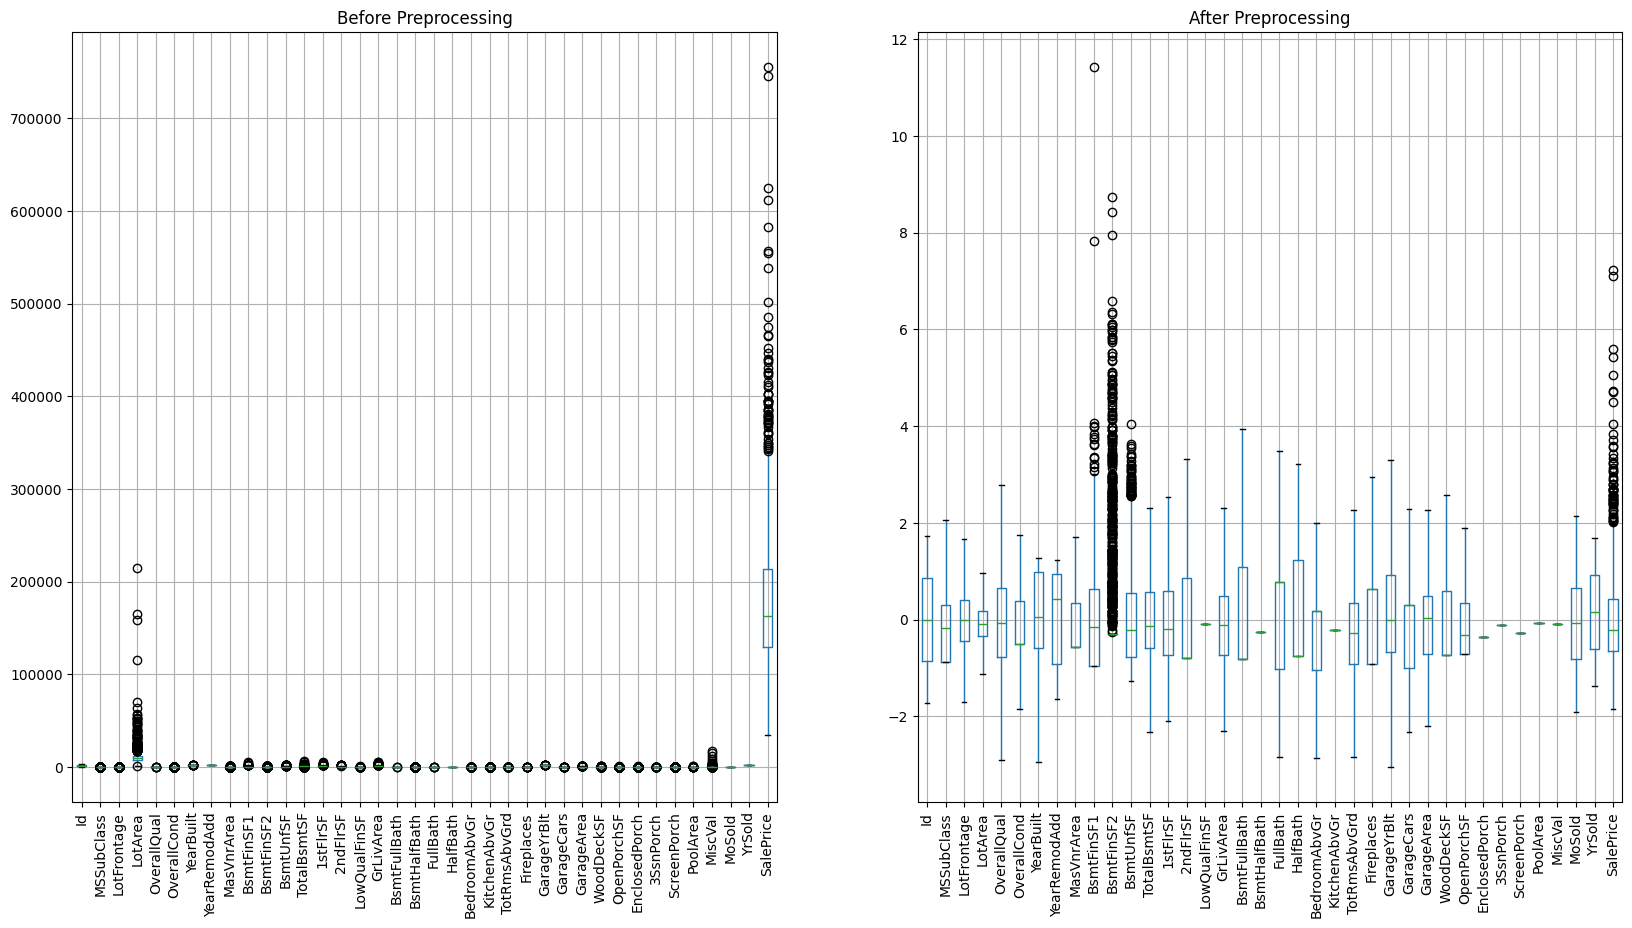
\includegraphics[width=1\textwidth]{media/comparison_house_prices.png}
%     \caption{Visualization of the data distribution before and after preprocessing}\label{fig:comparison-house-prices}
% \end{figure}

% \subsubsection{Iris Dataset}
% For the \textbf{manual approaches}, both the one by Shoukat Khan and our team
% started by loading the dataset, dropping the 'Id' column, and checking for null
% values and duplicates (with no duplicates or missing values found). This
% indicates a methodical approach to data cleaning. They used the StandardScaler
% method to scale numerical features, ensuring that data was standardized before
% applying any models. Both methods split the dataset into training and testing
% sets for further analysis, suggesting a consistent emphasis on validating model
% performance.\\ 
% The \textbf{AI-Driven Approaches} (Llama-based and
% application-driven ones) relied heavily on automation, which made preprocessing
% faster and consistent. Despite the simplicity of the Iris dataset, they
% effectively handled essential preprocessing steps, such as normalization and
% addressing potential issues like missing data (even though minimal issues were
% present). Both approaches excelled with simpler datasets like the Iris dataset,
% indicating that their strength lies in handling routine preprocessing tasks
% efficiently without much need for human intervention.\\ 
% In conclusion, manual
% approaches offered greater control and flexibility, allowing for a deeper
% understanding of the data, exploratory analysis, and custom preprocessing
% steps. On the other hand, the AI-driven methods focused on automating tasks to
% save time and reduce human effort, at the expense of adaptability and tailored
% transformations. In fact, manual methods are better suited to more complex data
% scenarios, as they allow for customization and tailored adjustments based on
% data insights, while AI-driven methods may be less flexible, especially for
% edge cases, and often require human oversight when facing unexpected data
% patterns.

% \begin{figure}[H]
%     \centering
%     \includegraphics[width=1\textwidth]{media/comparison_iris.jpg}
%     \caption{Visualization of the data distribution before and after preprocessing}\label{fig:comparison-iris}
% \end{figure}

\subsubsection{House Prices Dataset}

All the \textbf{manual approaches} carefully identify and impute missing data,
ensuring no data loss while maintaining data integrity. Different imputation
strategies are used based on context, with median or mean imputation for
numerical features and domain-driven values for categorical features. They all
transform categorical variables into numerical formats through one-hot
encoding, label encoding, or factorization. This ensures that the data is in a
form suitable for machine learning models. Alexandru Papiu and Erik Bruin
emphasize encoding of ordinal features using ordinal integers when applicable,
demonstrating consistency in preprocessing steps for such data types. Outliers
are identified and removed, and distributions of target and input features are
analyzed (e.g., via visual inspection). Both our team and Erik Bruin utilize
exploratory analysis, such as plotting distributions, to better understand data
trends and relationships between features.

Alexandru Papiu applies a log transformation to the target variable (SalePrice)
to reduce skewness, aligning it more closely with a normal distribution. The
Team's approach involves standardizing numerical features using StandardScaler,
a common practice to improve model convergence. This step was not mentioned in
the summaries of the other manual approaches but remains a potential
consideration for enhancing the comparability of numeric inputs.\\

Both \textbf{AI-driven approaches} involve automated code generation based on
input prompts, leveraging the capabilities of large language models (LLMs) to
understand and perform preprocessing tasks. The use of role prompting in Qwen2.5
guides it to generate tailored responses, demonstrating the value of carefully
constructed prompts in directing AI behavior.

The AI approaches automate typical preprocessing tasks such as imputation,
normalization, and encoding of categorical variables. The focus on basic data
cleaning, normalization, and transforming features for compatibility with
machine learning models shows their potential to streamline preprocessing
tasks.\\

Manual approaches demonstrate a nuanced understanding of data context. For
example, Erik Bruin groups related features for handling (e.g., Pool, Garage,
and Basement), applies specific imputation strategies based on domain
knowledge, and tailors transformations according to feature distributions.
AI-driven methods tend to follow generalized rules or learned heuristics, which
may not account for specific domain considerations without further tuning and
guidance.

Manual methods allow for fine-tuning based on data insights gained from
exploration, such as identifying and removing outliers, specific imputation
strategies, and encoding schemes tailored to data distributions. AI-driven
methods using Qwen2.5 and LLaMA often require human intervention to refine the generated
code, demonstrating limitations in achieving optimal solutions without manual
oversight.

AI approaches offer a faster, automated process for generating initial
preprocessing scripts, reducing the amount of repetitive work required by data
scientists. This can be highly beneficial for rapid prototyping. Manual
approaches are more time-consuming but can be more precise due to direct human
involvement and domain knowledge.

Manual methods generally exhibit fewer errors because they leverage human expertise to identify and address issues during each preprocessing step. In contrast, AI-driven preprocessing, such as that performed by Qwen2.5, often produces code that can be suboptimal or contain errors without substantial human refinement. In our experiment, the LLM's output was often insufficiently accurate, remaining overly generic and requiring numerous iterations to yield a functional solution. Even then, the results fell short of the quality expected for reliable preprocessing. This highlighted a significant gap in the model's ability to autonomously make effective decisions, underscoring the need for substantial improvement before it can be considered a viable alternative to human-led preprocessing in complex scenarios.

\begin{figure}[H]
    \centering
    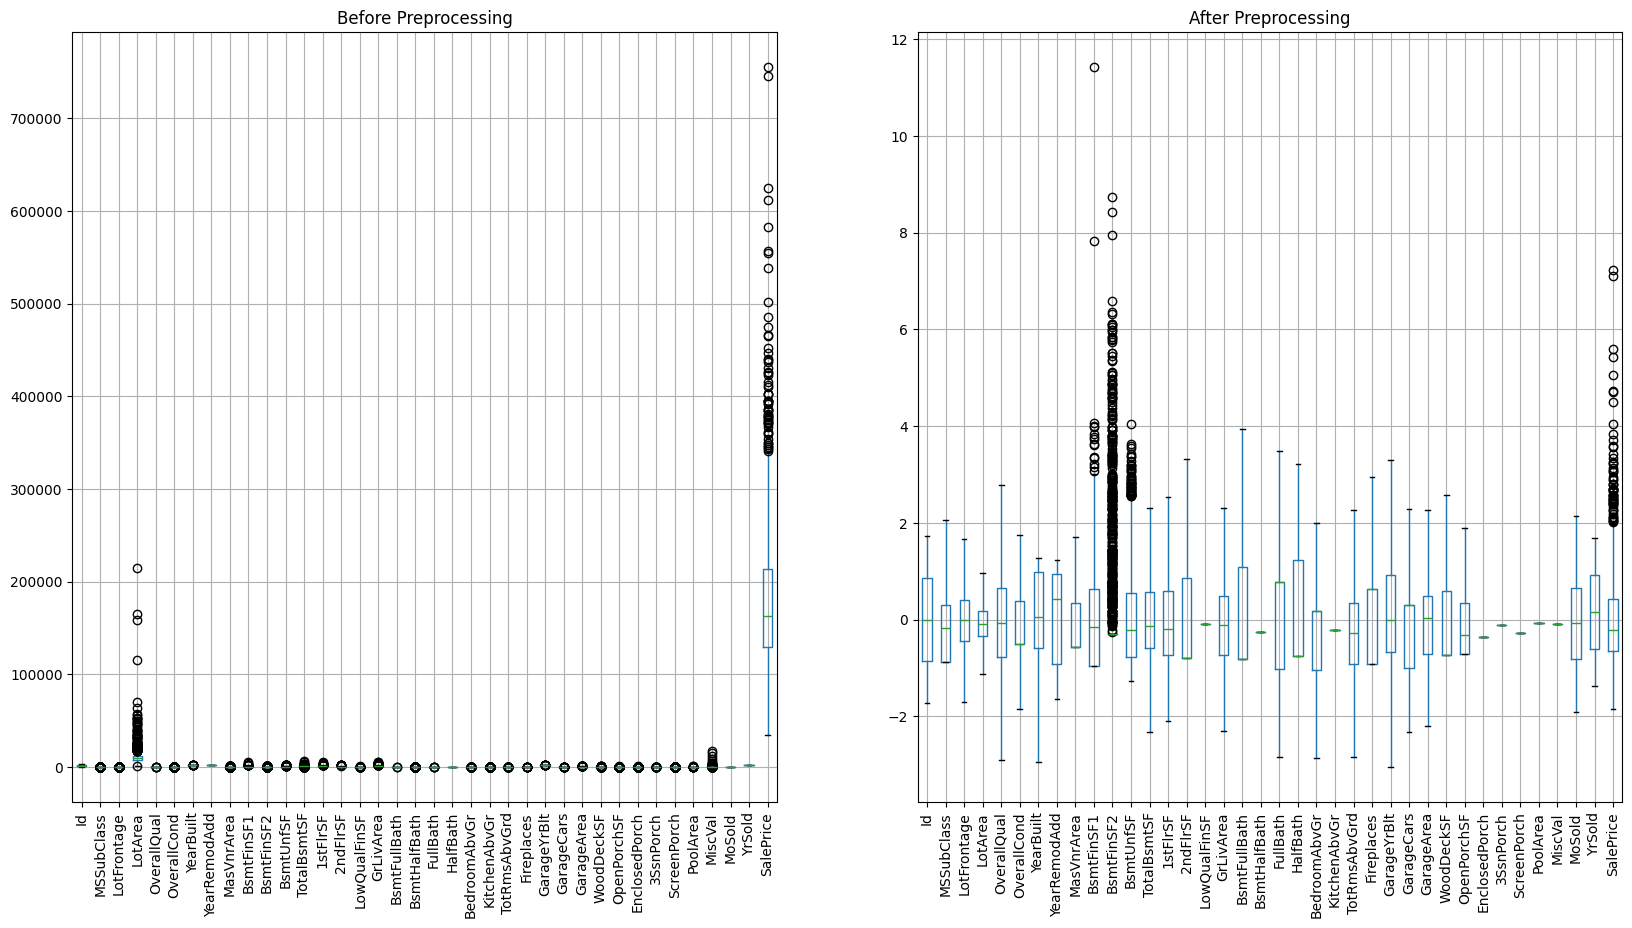
\includegraphics[width=1\textwidth]{media/comparison_house_prices.png}
    \caption{Visualization of the data distribution before and after preprocessing}\label{fig:comparison-house-prices}
\end{figure}

\subsubsection{Iris Dataset}
For the \textbf{manual approaches}, both the one by Shoukat Khan and our team
started by loading the dataset, dropping the 'Id' column, and checking for null
values and duplicates (with no duplicates or missing values found). This
indicates a methodical approach to data cleaning. They used the StandardScaler
method to scale numerical features, ensuring that data was standardized before
applying any models. Both methods split the dataset into training and testing
sets for further analysis, suggesting a consistent emphasis on validating model
performance.\\ 
The \textbf{AI-Driven Approaches} (Qwen2.5 and Llama-based) 
relied heavily on automation, which made preprocessing faster and 
consistent. Despite the simplicity of the Iris dataset, they
effectively handled essential preprocessing steps, such as normalization and
addressing potential issues like missing data (even though minimal issues were
present). Both approaches excelled with simpler datasets like the Iris dataset,
indicating that their strength lies in handling routine preprocessing tasks
efficiently without much need for human intervention.\\ 
In conclusion, manual
approaches offered greater control and flexibility, allowing for a deeper
understanding of the data, exploratory analysis, and custom preprocessing
steps. On the other hand, the AI-driven methods focused on automating tasks to
save time and reduce human effort, at the expense of adaptability and tailored
transformations. In fact, manual methods are better suited to more complex data
scenarios, as they allow for customization and tailored adjustments based on
data insights, while AI-driven methods may be less flexible, especially for
edge cases, and often require human oversight when facing unexpected data
patterns.

\begin{figure}[H]
    \centering
    \includegraphics[width=1\textwidth]{media/comparison_iris.jpg}
    \caption{Visualization of the data distribution before and after preprocessing}\label{fig:comparison-iris}
\end{figure}
\chapter{Conclusion}

The results of this experiment indicate that automating the data preprocessing phase using Qwen2.5 shows promise, particularly with simpler and smaller datasets. In the case of the \textit{Iris} dataset, which is relatively straightforward, the approach demonstrated the potential for generating Python code that performs several essential preprocessing tasks. However, when faced with more complex datasets, the results were less satisfactory. The LLM was not able to fully meet the preprocessing requirements in terms of accuracy and completeness, because of the challenges of handling larger, more varied datasets.

While the performance of Qwen2.5 in this experiment did not reach the desired level for all use cases, it is crucial to emphasize that the idea behind automating data preprocessing is highly feasible. The current limitations of the results should not overshadow the potential of this approach. In fact, the experiment has proven that, with improved focus and enhanced methodologies, it is possible to develop a system capable of automating data preprocessing with higher accuracy and efficiency.

One promising method to improve preprocessing automation would be to iterate the process multiple times on the same dataset. After each round of preprocessing, the model would be provided with new information from the partially preprocessed dataset, which could be used to refine subsequent preprocessing tasks. This iterative approach would allow the system to progressively improve its understanding of the dataset and make more informed decisions in later stages of preprocessing. This could potentially lead to a more robust and effective preprocessing pipeline, where each iteration builds on the insights gained from previous steps.

The future of this concept is particularly exciting when considering the growing capabilities of LLMs and other machine learning models. By fine-tuning these models specifically for data preprocessing tasks and leveraging more powerful computational resources, it is likely that significant improvements can be made. With specialized models designed for this purpose, the accuracy and efficiency of the automated preprocessing workflow can be greatly enhanced, making it a viable solution even for complex datasets.

From a business perspective, the automation of data preprocessing holds significant promise. In many industries, data is the cornerstone of decision-making, but the preprocessing phase is time-consuming, labor-intensive, and often prone to human error. Automating this phase would not only reduce the amount of time spent on repetitive tasks but also allow data scientists and analysts to focus their efforts on higher-level tasks, such as model development and strategic decision-making. By reducing the manual effort required in preprocessing, companies could benefit from increased productivity and more efficient use of their workforce.

Moreover, the time saved during preprocessing could lead to faster project turnaround times. This can be especially important in industries where timely insights are critical, such as finance, healthcare, and marketing. The automation of preprocessing could also lower operational costs, as fewer resources would be required for data cleaning and preparation. Additionally, with a more consistent and error-free data preparation process, the risk of producing misleading or inaccurate analysis could be minimized, leading to more reliable decision-making.

The ability to automate data preprocessing could also enhance the competitiveness of companies that adopt it. By streamlining data workflows and reducing the time between data collection and analysis, organizations could move more quickly in responding to market trends and customer needs. This agility is crucial in today's fast-paced business environment, where gaining a competitive edge often depends on the speed and accuracy with which data is processed and analyzed.

In conclusion, while the results of this experiment may not have reached the desired level of performance with more complex datasets, the potential for using Qwen2.5 to automate data preprocessing is enormous. With continued advancements in computational power, model specialization, fine-tuning and in using more advanced versions of Qwen2.5, this approach could become a key tool for businesses looking to optimize their data workflows. The advantages in terms of cost savings, increased efficiency, scalability, and competitive advantage make this a highly promising area for further exploration and investment. Automating data preprocessing could ultimately transform the way businesses handle their data, empowering them to make faster, more informed decisions while reducing operational overhead.

\section{Future Work}

% The results of this experiment provide a strong foundation for further exploration in the field of automating data preprocessing using large language models (LLMs). However, to achieve more robust and reliable outcomes, several key areas for future work should be prioritized.

% First, model fine-tuning stands out as a crucial next step. Qwen2.5, being a general-purpose language model, does not fully capture the domain-specific nuances of data preprocessing tasks. Fine-tuning it on domain-specific datasets, particularly those focused on data preprocessing, could enhance its ability to handle the complexities of larger and more varied datasets. A model trained with a more targeted set of preprocessing scenarios and solutions would likely demonstrate improved performance in more complex situations.

% Additionally, hyperparameter optimization could improve model performance significantly. Experimenting with different hyperparameters and model configurations can lead to better adaptation to specific applications and datasets, improving the overall accuracy and efficiency of preprocessing tasks.

% Another promising avenue is the development of an iterative preprocessing approach, where the model refines the dataset progressively over multiple rounds. After each preprocessing step, the model would be provided with new information from the partially preprocessed dataset, allowing it to adjust and improve its strategy in subsequent rounds. This iterative process could greatly enhance data quality, as each step would build upon insights from previous iterations, enabling the system to make more informed decisions and address data issues more comprehensively.

% Moreover, the integration of other models into the preprocessing pipeline could provide performance benefits. Using ensemble methods or combining the Qwen2.5.5 model with other state-of-the-art models may enhance preprocessing by leveraging the strengths of different approaches. This could result in better handling of complex tasks and improve overall system robustness.

% Addressing the limitations of computational resources is another important factor. As the model grows in complexity, leveraging more powerful hardware and optimized algorithms will be essential to improve the speed and efficiency of preprocessing tasks. As computational capabilities advance, the performance of LLMs in handling larger and more complex datasets will likely improve, making the approach more scalable and efficient.

% In addition, there is a need for research into automating feature engineering and improving the handling of missing, inconsistent, or erroneous data. 

% Furthermore, user feedback incorporation should be considered for future iterations. By developing mechanisms that allow for the inclusion of user feedback into the preprocessing pipeline, the system can continuously improve based on real-world needs and user experience. 

% Finally, the integration of this automated preprocessing system into existing data pipelines is a crucial next step. Embedding this system into business workflows will allow organizations to realize the full potential of automated data preparation, creating a seamless and efficient end-to-end process. As businesses look to scale their data operations, integrating such automation could help reduce the burden of manual data preparation, accelerating the entire data processing pipeline.

In summary, while the current experiment offers a promising proof of concept, future work should focus on improving the model's ability to handle complex datasets, incorporating iterative preprocessing techniques, fine-tuning the model for domain-specific tasks, and addressing computational and integration challenges. The addition of features like hyperparameter optimization, user feedback loops, and ensemble modeling approaches will further enhance performance. With continued advancements in AI-driven automation, the potential for fully automating the data preprocessing phase holds great promise, offering substantial business benefits in terms of efficiency, consistency, cost reduction, and scalability.

%\subsection{Future Work}

%While the results obtained are promising, they indicate potential for further improvement. Future work could focus on several key areas:

%\begin{itemize}
    %\item \textbf{Model Fine-tuning}: Enhancing the model's performance through additional fine-tuning on domain-specific datasets could yield better accuracy and efficiency in preprocessing tasks.
    
    %\item \textbf{Hyperparameter Optimization}: Experimenting with different hyperparameters and model configurations may improve performance metrics and adapt the model more effectively to specific applications.
    
    %\item \textbf{Integration with Other Models}: Exploring the use of ensemble methods or combining Qwen2.5.5 with other state-of-the-art models could enhance performance through the benefits of diverse modeling approaches.
    
    %\item \textbf{User Feedback Incorporation}: Developing a mechanism to incorporate user feedback into the preprocessing pipeline can lead to iterative improvements, making the application more responsive to real-world needs.
    
    %\item \textbf{Extended Features}: Adding more preprocessing functionalities, such as advanced text augmentation techniques and context-aware normalization, could significantly enhance data quality and usability.
%\end{itemize}

%Overall, this project demonstrates the potential of using advanced language models like Qwen2.5.5 in real-world applications. By automating critical phases such as data preprocessing, we can improve efficiency, maintain consistency, and ensure data privacy, which is fundamental for firms. The open-source nature of Qwen2.5.5 fosters collaboration and innovation within the community, paving the way for further advancements in natural language processing and machine learning.

\end{document}
